\documentclass[a4paper]{report}

% Packages
\usepackage{enumitem}
\usepackage{graphicx}
\usepackage{array}
\usepackage{float}
\usepackage{url}
\usepackage[maxbibnames=5,style=numeric,backend=bibtex,sorting=nty,firstinits=true]{biblatex} \bibliography{ref}
\usepackage[noabbrev,capitalise]{cleveref} 
\usepackage{tabularx}
\usepackage{tabu}
\usepackage{longtable}
\usepackage[british]{babel}
\usepackage[font=footnotesize]{caption}
\usepackage{csquotes}
\usepackage{color}
\usepackage{rotating}

% Settings
% Margins in lists
\setlist[itemize]{noitemsep}
\setlist[enumerate]{noitemsep}
% Margins in tables
\renewcommand{\arraystretch}{1.3}

% Text replacement commands
\newcommand{\ie}{i.e.,}
\newcommand{\eg}{e.g.,}
\newcommand{\IVF}{IVF}
\newcommand{\PRN}{PRN}
\newcommand{\AMC}{AMC}
\newcommand{\project}{IVF-PRN project}
\newcommand{\ivfsystem}{IVF-PRN system}
\newcommand{\escience}{e-Science}

% Commenting commands
\newcommand{\silvia}[1]{\textcolor{red}{\textbf{*Silvia: }\textit{#1}}}
\newcommand{\allard}[1]{\textcolor{red}{\textbf{*Allard: }\textit{#1}}}
\newcommand{\note}[1]{\textcolor{cyan}{\textit{#1}}}

%\title{Developing a Data Management System for Obstetric Research Into Long Term Effect of In Vitro Fertilisation Techniques}
\title{A Data Management System for Obstetric Research}

\author{
	Allard J. van Altena\\
	University of Amsterdam\\
	Email: a.j.vanaltena@amc.uva.nl
}

\begin{document}

%	\maketitle
	
	\tableofcontents
	
	\chapter{Introduction}
	\label{introduction}

	%TODO: Check if terminology is explained, IVF, PRN, clinical audit registration, \ivfsystem{}, \project.
	
	\paragraph{The domain and background}
Reproduction is a fundamental building block of life.
For the human species this means that two individuals, with a different sex each, produce offspring.
The offspring contains the genetic material of both the parents.
However, there are many conditions and diseases which can lead to infertility or subfertility.
In the Netherlands these terms are defined in a national guideline by the Dutch association of obstetrics and gynaecology (NVOG)\footnote{Dutch: Nederlandse vereniging voor obsetrie en gynaecologie}\cite{subfertilityGuideline}.
Infertility being defined as a rare condition where ``no chance of reproduction exists''.
And subfertility as ``failure to become pregnant after twelve months of unprotected coitus aimed at conception''.
Approximately 5\% to 8\% of all couples remain without children unwillingly \cite{cbsStatistics, nhgStatistics}.

Luckily there are several fertility treatments.
Some of these lead to both the parents becoming biological parents. 
Others make use of donor material or surrogates, meaning that the child does not contain the genetic material of one of the `parents'.
Commonly used treatments include intrauterine insemination (IUI) and in vitro fertilisation (IVF) \cite{treatmentExplanation}.
Of these IUI is closer to regular impregnation, as sperm cells are collected and injected deep in the uterus, while IVF happens `in vitro', \ie{} in glass, outside of the body.
IVF can be further divided into more specific treatment types (\eg{} intracytoplasmic sperm injection, ICSI), 
the difference between these being the used technique or the type of parental materials used.
For example, there are fresh and frozen treatments; in a frozen treatment, material of the male or female is kept in (frozen) storage before being used.
Nevertheless, each treatment follows about the same steps: egg maturation stimulation, egg retrieval, fertilisation, and embryo transfer \cite{treatmentExplanation}.
The stimulation phase can also be called the start of a new \emph{cycle}. In The Netherlands (according to the NVOG) 14,562 of these cycli were started in 2013 \cite{ivfReportNVOG2013}, approximately 30\% of which resulted in a ongoing pregnancy.
The success rate for a given fertility clinic is fairly well known.
However, outcome quality indicators related to the (born) child are either sparse or unknown.

All births in the Netherlands have to be entered into the perinatal registry (perinatale registratie Nederland, \PRN{}\footnote{http://www.perinatreg.nl}).
For research purposes, however, this data is completely separated from the clinic's patient data.
The Dutch healthcare system is quite exceptional as fertility clinics are in the public domain, 
meaning that there is pressure for disclosing  data for research and governance reasons.

With minimal identifying data from both the fertility clinics and the \PRN{}, treatment input and outcome can be linked together.
To execute this linkage the \project{} was established \silvia{[reference?]} \allard{asked Martina: TODO}.
During the project, data between 1999 and 2010 is gathered from each of the thirteen Dutch fertility clinics and linked to the \PRN{}.
This data covers only ongoing pregnancies, as a child has to be born in order to link to the \PRN{}.
In the given date range about 44,164 ongoing pregnancies were registered in the clinic data \cite{ivfReportNVOG}.
Linkage will inevitably result in a loss of a few percent where no appropriate match can be found.
But a considerate amount of pregnancies is available for research.
The linkage part of the research is outside of the scope of this paper and will be provided by another project.
	\paragraph{What is big data?}
With the buzzword `big data' people often associate terms like size, volume, and analytics.
However, there are a lot of other data manipulation challenges that can lead to data being classified as ``big ''.
McAfee \cite{dsb1mcafee} describes big data as lots of data coming in at a high pace from many different sources, in large `volume, velocity, variety'.
Jacobs \cite{dsb5jacobs} presents it from a changing perspective of technical possibilities.
In the 1980s 100GB of data was considered big, but now the perspective has changed: what you try to do with the data makes it big or not.
Lynch \cite{dsb3lynch} stresses the problem of `lasting' (big data preservation), \ie{} how do we model and preserve the registered (sometimes unique) events.

There are wide gaps between these definitions but also similarities.
One overarching idea about big data is that it can help understand specific domains and help make decisions \cite{dsb2lohr}.
Jacobs even states that transactions and storage of data are already largely solved problems \cite{dsb5jacobs}.
This leaves decision making, modelling, and preservation as the main remaining challenges.

Big data in the corporate world mostly means management and quick reaction to real life events.
A good example is flu prediction: Google is a week faster in predicting hospital visits related to flu than the official government sources \cite{dsb8dugas, dsb1mcafee}.
McAfee~\cite{dsb1mcafee} even states that ``Data-driven decisions are better than expert-opinion decisions''.

As decisions are based on the interpretation of the data, modelling of data should reflect events in the real world.
To make the event interpretable to the machine, the event should be recorded in a structured manner.
Recording and keeping this data from events for long periods of time, such that it can be used for decision making, is the last challenge of preservation.
For example, losing data can be of significance as each event is unique and will not occur again in the same way.
There are also side effects: keeping any data (specifically medical) about persons raises many privacy challenges \cite{dsb1mcafee}.

\paragraph{Big data for \project{} research}
The \project{} dataset (\projectdata{}) consists of linked data from \IVF{}-clinics and the \PRN{}.
In the context of the \projectdata{} two of the big data factors lead to challenges: decision making and preservation.
These are mainly human related or procedural, \eg{} ethics, trust, expectancy, lack of organisational support, etc.
Modelling of data is (currently) quite straightforward, as mainly data has to be ready as input material for popular statistical software like SPSS \cite{spssSoftware} or R \cite{rSoftware}.
Introducing this model to computerised decision making may result in semantic or metadata problems, but compared to the other challenges these can be handled quite easily.

Currently researchers make decisions on many levels, \eg{} what relevant hypotheses exist, which research hypothesis to pursue, what data should be analysed, how data should be interpreted.
Many of these decisions can be supported with computerised systems.
For example, a hypothesis ``sweep'' can be executed with data mining operations, finding correlation in the data.
However, many clinical researchers hold on to generation of hypothesis based on expertise, possibly leading to missed (important) conclusions.
This might describe a trust or expectancy issue with computerised systems, or the actual value of such a data mining system was never demonstrated in practice.

On the other hand are the problems preservation poses.
Funding bodies demand more of researchers considering data-management and sharing \cite{dsb3lynch}.
These demands can even extend beyond the duration of the funding, resulting in long lasting storage issues but also providing more opportunities for reuse.
For individual research projects this can be problematic as decisions on this level should be made at a institutional control \cite{dsb3lynch}.
In this project, because assisted pregnancies are relatively rare and data gathering is a troublesome process, reuse should be encouraged to make the effort useful and significant.

Lastly, preservation and reuse of data will also throw up barriers for the data deliverers.
Right now success percentages of clinics are being published as this is required by law, however they complain that the patient mix between clinics is unfair.
Clinics want to cooperate in the \project{} but they are afraid that research outcomes will be published in a way that will reflect directly on individual clinics. 
Trust needs to be gained by all the actors involved to fully exploit the value of the \project{}.

%3 - Big data- How do your data grow?
%It also includes defining and recording appropriate metadata — such as experimental parameters and set-up — to allow for data interpretation
%This is best done when the data are captured. Indeed, descriptive metadata are often integrated within the experimental design. Description includes tracing provenance 

%1 - Big data the management revolution
%Perhaps even more important are skills in cleaning and organizing large data sets; the new kinds of data rarely come in structured formats. Visualization tools and techniques are also increasing in value.
%The best data scientists are also comfortable speaking the language of business and helping leaders reformulate their challenges in ways that big data can tackle
%The technologies are new and in some cases exotic. 
%It's too easy to mistake correlation for causation and to find misleading patterns in the data. 
%few things are more powerful for changing a decision-making culture than seeing a senior executive concede when data have disproved a hunch.
%They'll be valued not for their HiPPO-style answers but because they know what questions to ask
%When it comes to knowing which problems to tackle, of course, domain expertise remains critical
%Big data's power does not erase the need for vision or human insight.
	\paragraph{Using IT as leverage}
Summarising, the challenges come down to a change of attitude.
Even though literature describes big data as a benefit for the users, medical researchers are shying away from using it.
How can they be convinced that following certain big data guidelines can evolve performing research itself?

This work shows a proposal for a supportive system which can manage data produced by the \project{}; its working name is: \project{} Research Gateway (\ivfsystem{}).
It is meant to show what value can be delivered if some human performed functions are left for a computerised system in the management of such a valuable and sensitive dataset.
In order to give direction to the development, the following main aspects have been investigated: security, data access, data browsing, and data querying.
This resulted in the following research questions:

\begin{enumerate}
	\item How do we implement a user-friendly system in a IVF medical domain which covers problems concerning: data security, data access, data browsing, and data querying?
	\item What needs to be changed in the current attitude towards data usage to promote big data in a IVF medical domain?
\end{enumerate}

These two questions were broken down into sub questions. 
For question 1:
\begin{itemize}
	\item What are the functions of this system and which parts of the research process should this system support?
	\item Who are the users and what are the use cases for these users?
	\item What are the legal and security aspects of this system?
	\item What is the data model for this system?
	%\item What functions were actually implemented in the prototype? \silvia{this is no research question. maybe 'what is a minimum prototype to demonstrate ...'}
	\item What is the minimum prototype demonstrating that the system's goals are reachable? \allard{?}
	\item To what extent does this system meet the expectations of users?
\end{itemize}

For question 2:
\begin{itemize}
	\item What are the blocking aspects of data usage?
	\item What are the promoting aspects of data usage?
	\item What alignment needs to take place to promote data usage?
	\item How can IT be leveraged to achieve this goal?
\end{itemize}
	
	\chapter{Requirement Analysis}
	\label{requirements}
	
	in this chapter ...
first this, then that


\silvia{general notes: 
\\(1) need to give a name for the dataset "fertility data repository"? ivf/prn repo? ivf-repo something short that you can simply use in this section.
\\(2) also need a name for the SG that is the main object in the thesis. 
the terminology should be introduced in the intro and used consistently afterwards
}

\section{Process Analysis}
\label{process-analysis}


\paragraph{Research workflow}
When doing research in the medical domain a well known workflow is often used. Nwogu \cite{nwogu} has formally described and defined this workflow for scientific reporting purposes (\ie{} writing scientific papers).
Figure \ref{fig:research-workflow} shows the simplification of this workflow, which includes problem definition, formulation of research question, definition of methods, data aquisition, data analysis, statistical analysis and conclusions. \silvia{i dont understand "outcomes" - does it mean stats? or results?}

Clinical research (\eg{} a trial) is well suited to follow this workflow, as each step can be executed in turn and data acquisition is often the most time-consuming part.
However, acquisition of new data is not always necessary,  desirable or even possible. 
\silvia{ "with the rise of cheap disk space and big data this does not have to be true" - this is not the motivation. data is valuable and needs to be reused, this is the motivation.}
Research data of high quality and trustworthiness can be preserved and re-used endlessly, upon well controlled conditions. 
This is the case of IVF-repo.

\paragraph{Research Workflow using the IVF-repo}
In the \project{} considerable time has been spend on gathering valuable data. The goal of this SG is to facilitate reuse of this data. 
There is, however, one major restriction with data sharing and re-use: medical data is (almost always) highly sensitive and must be secured. 
This imposes strong conditions for reusing the data, which needs to be taken into account by the system.


\begin{figure}[hb]
	\centering
	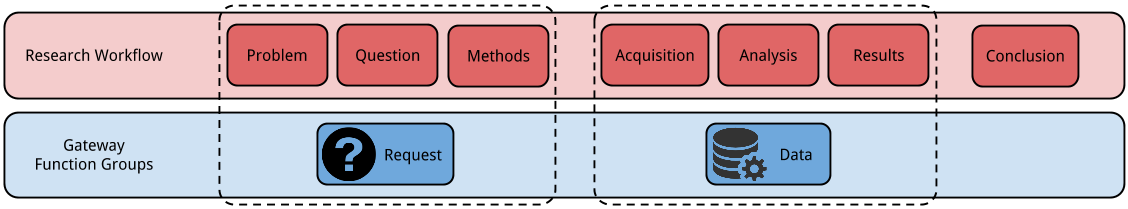
\includegraphics[width=1.0\linewidth]{images/research-workflow}
	\caption{
		This figure shows a simplification of the research workflow often used  in the medical domain (based on \cite{nwogu}).
		The workflow building blocks are mapped by the identified system function groups. Note that the data acquisition block requires execution of acquisition methods from the methods block.
	}
	\label{fig:research-workflow}
\end{figure}

\silvia{put something saying that the SG will support this process, in a case where data acquisition is actually done by consulting the XXX data repository. researchers need to find data, request it, get permission, receive the data. data managers need to keep track of all actions. 
also explain and how you move on to detail from here (functionality design)}

\section{Initial concept}

\silvia{i think this should be a separate section. give it a name (seed concept? seed design?) - just "seed" is not enough. There was also some study done prior to this design (interviews, study, observation).
briefly report this in 2.1. Then you can present the first design itself (fig 2.1)}

Restricting the use of data to one user is undesirable, therefore good data management has to be applied to enable re-use.
\silvia{explain where the initial idea came from (maybe this is the link with the previous part?}
The initial idea in this project was to develop a data management system with data-centric functions, \eg{} request, upload, download, search.
These are represented in figure \ref{fig:research-workflow} with the blocks `request' and `data'.
With these functions a big part of the research workflow would be supported.


\silvia{
this was at the caption, but i think it should not. captions are used to explain the figure - nothing else. generic stuff goes to the text body:
External services such as .. are provided ?? and outside of the scope of this paper.
Two direct users and several external users are planned each with their specific set of functions.
		Data listed is either available at initialisation of the system or is generated during execution.
}
		
\begin{figure}[t]
	\centering
	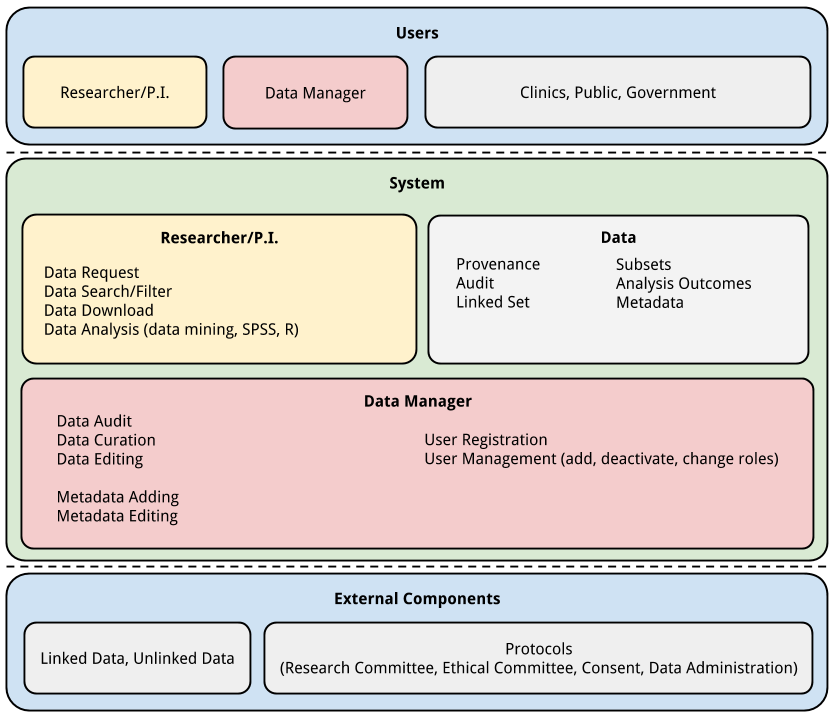
\includegraphics[width=1.0\linewidth]{images/brainstorm-before}
	\caption{
		Initial concept for the \ivfsystem{}, encompassing data and user management. 
		3 user roles (a,b,c, indicated by colors. system offers different set of fuctions for each role.
		system has access to external services to obtain data
	}
	\label{fig:brainstorm-before}
\end{figure}

Figure \ref{fig:brainstorm-before} describes the full view of the seed, the function groups are expanded into: users, external services, data, and functions.
The external services are of influence on the system but are outside of the scope of this paper.
Meaning that data and protocols (necessary for lawful execution of the system) are already provided.
From the provided data unlinked data is \project{} data split into clinics and PRN, where linked data are the matched rows from both.
Projected direct users are researchers and data managers.
Furthermore, external parties (clinics, public, government) might be interested in statistics of the system and its data, \eg{} aggregated and anonymised analysis outcomes.

Functions for each of the users encompass data management and user management.
Data functions meaning mutations of the raw \project{} data, where metadata is metadata of this raw data.
The data block refers to data being stored in the system at initialisation and during execution.
The linked set (\ie{} raw data) is an initialisation input of the system.
Other items are generated during execution, \eg{} subsets are created after a data request is granted which also results in provenance data, etc.
	
	\section{Brainstorm}
\label{brainstorm}

A brainstorm session was organised with key stakeholders to discuss the initial concept.
The stakeholders were spread over the different potential end-users: researcher, principal investigator, data manager, research committee.
The goal of this session was to evaluate the initial concept, which is described in the previous section, and to find any `hidden' functions that were not apparent during the observations.

\paragraph{The execution}
Brainstorming is not an exact science, therefore there is no pre-defined schema to follow.
However, there are a lot of gurus describing guidelines to manage sessions.
The following list is an implementation of guidelines taken from Tyner Blain \cite{brainstormWebsite}:

\begin{enumerate}
	\item \textbf{Rules -} Make sure everyone is on the same level and understands what the point of the meeting is through a small introduction talk.
	\item \textbf{Time limit -} Guidelines describe short sessions, but due to the complexity of the system two sessions of one hour each were necessary.
		Step 3 (seed) was repeated in the second session to refresh the idea of the system for everyone.
	\item \textbf{Starting point -} In this case the initial concept described in section \ref{process-analysis} was used as a starting point.
		During the session big (A2) pieces of paper were used on which the seed's functions are written down. Figure \ref{fig:brainstorm-before} is a stylised version of the used paper schema.
	\item \textbf{Ideas -} The sessions are structured by the paper schema, each of the functions is discussed.
		Ideas for new functionality or differences are shortly (vocally) summarised by the session leader (in this case the researcher) and written on the same paper.
	\item \textbf{Prioritise -} For this step the guidelines are disregarded and prioritisation is based on group agreement.
		Three levels are used: must have, should have, nice to have.
		Any functions that are deemed unnecessary were already removed from the schema during the `ideas' step.
\end{enumerate}

\paragraph{Results: differences}
Outcomes of the brainstorm showed that many requirements were hidden when the initial concept was defined.
The revised complete research life cycle for the \project{} is:
\begin{itemize}
	\item researcher submits a data request;
	\item committee members check this request and either approve it or not;
	\item the system creates a subset of data which the researcher can access;
	\item after completion of the research the researcher uploads his/her paper;
	\item the committee members check this paper and either approves it or not;
	\item during the whole cycle the data manager keeps an overview of this process.
\end{itemize}

This whole cycle is to be supported by the \ivfsystem{}.
There are a couple of differences with the initial concept.
The first being that researchers should be allowed to register themselves into the system with a limited account (\ie{} no access to data, no data requests).
After registering, the data manager is responsible for approving their account.

Then the second difference shows, namely, the data request approval process will also reside in the system.
As said before, a request is a document which contains information the research committee needs to base their decision on.
This information in the case of the \ivfsystem{} is: research question, hypothesis, problem background, description of perceived methods to solve question, and the requested data.
The document is formulated by the researcher and after submission, managed by research committee members (\ie{} evaluated, voted on).

After the researcher has access to his/her data the next difference become apparent.
The stakeholders representing the researchers said that analysis will mostly be done offline.
They are known and comfortable with the software they are using and are unwilling to switch.

This brings us to the next difference, data is not to be downloaded over the internet due to privacy reasons. 
Access should be restricted such that only certain (physical) places have direct access to the \projectdata{}.
However, metadata such as a data dictionary (\ie{} a document describing what data is available in the repository) can be accessed over the internet.
This helps the researcher in formulating their data request and provides more opportunity for data reuse (\eg{} someone might be unwilling to travel long distances just to submit a request).

The last step in the research life cycle, the publication, should also be supported in the system.
Publications have to be approved by the research committee before they can be published.
As with the data request process, the researcher creates a document (\ie{} upload a paper to the system) which is evaluated and approved by the committee.

Lastly, two notable differences outside of the research life cycle.
No third parties should be allowed on the system, for now the data is too valuable and studying exactly what information can be passed on is not a priority.
Secondly, no unlinked data will be stored or used in the system.
It might be interesting to find correlations between linked and unlinked data, but that is not the goal of the \project{}.

The focus of the system switches from purely data support to also supporting other research related tasks.
This is clearly visible in the revised workflow, figure \ref{fig:research-workflow-after}, which shows that the balance has shifted from just the `Data' group to a much broader perspective.

\begin{figure}[hb]
	\centering
	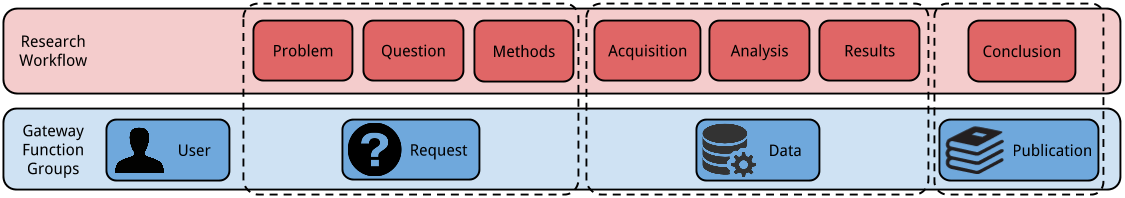
\includegraphics[width=1.0\linewidth]{images/research-workflow-after}
	\caption{
		Research workflow mapped by identified function groups after brainstorm, initial workflow shown in figure \ref{fig:research-workflow}.
		The user group underlays the whole system and is therefore outside of the dotted mapping lines.
	}
	\label{fig:research-workflow-after}
\end{figure}
	
	\clearpage

\section{Security}
\subsection{Literature Review}
\label{security-literature}

The question we seek to answer in this section is what regulations and conventions should be taken into account when storing and processing data specific to our \ivfsystem{}?
We could start with answering the question `how do I secure data?', but before doing this it is important to describe what the incentives are for using the data.
We do this to give context to the found security issues and proposed solutions for them.

\paragraph{Medical big data ethics and security}
\label{security-ethics}

In 2013 Groves \cite{s20Groves2013} estimated big data strategies could increase profits in US healthcare by \$100 billion \cite{s13Patil2014}.
However to make this possible healthcare management has to change their business model.
Old models worked with increasing or decreasing the amount of patients while the outcome (quality) remained the same; Patil \cite{s13Patil2014} calls these ``volume-based business models''.
To make the increase in profits possible, new models revolving around cost versus quality are used, called ``value-based business models''.
Much more is written about the pros and cons of this type of healthcare management by gurus like M.E. Porter \cite{s21Porter2006}, but this is outside the scope of this paper.

In order to measure the quality indicators in the new strategies big data can be applied \cite{s6West2009}. 
Through data mining, patient outcomes can be connected with treatment, environmental factors, or any other information.
When this is done right choosing the best treatment for any given new patient will be a matter of checking the charts.
This way of delivering healthcare is also supported by the European Union which describes it as ``Free Movement'' for patients between institutions, obtaining quality, and efficient healthcare \cite{s8FernandezAleman2013}.

The new set-up closely fits to a research set-up, in the sense that patient data is used for improving the healthcare process.
Data in patient records is mainly used to provide information for caretakers, but it can be very valuable in research as well \cite{s15Fenz2014}.
Because the current model of healthcare data is not fully compatible to the ``value-based business models'' extraction of data is not very straightforward.
Also, caution should be kept as there are security and privacy pitfalls.

Even though these problems exist, according to Fenz \cite{s15Fenz2014} patients will not withhold their data for research purposes.
However, there are concerns that data can be accessed by persons with unwanted intentions: marketing, insurance, or data loss through breaches.
It is a good thing that big data can help the improvement of healthcare \emph{and} patients are willing to give their data towards this end.
But data breaches should never be dismissed, which makes the application of big data an ethical question: Does the benefit of the big data overcome the possible negative effects of a data breach?

Kluge \cite{s7Kluge2007} looked into this ethical question by taking a context: ``What should be the driver of its [the systems'] development and implementation?''. 
And splitting the main question into four sub-questions, respectively: Should it be the technology itself? Should it be the interests of service providers? Should it be the interests of governments? Should it be the interests of patients?
Each of these questions are applicable to the \project{}:

\begin{itemize}
	\item \textbf{Should it be the technology itself? -} Because this system is developed in the interest of research, the technology has a stake in the driver of development.
	However, it should not become the main driver as a fully optimised system does not necessarily translate into improved quality and efficiency of care.
	Which, in an ethical sense, should always be the main driver as patient `donate' their data for this purpose.
	\item \textbf{Should it be the interests of service providers? -} If the \ivfsystem{} is implemented in a broad scope it should also include feedback.
	This is in the interest of the service providers (\ie{} clinics) as they will finally be able to get a impartial comparison between each other.
	If the feedback to providers is delivered in the right manner this should provide both the incentive \emph{and} the knowledge to improve efficiency.
	However, in the current scope of the \project{}, feedback is not accounted for.
	\item \textbf{Should it be the interests of governments? -} Because the \project{} is the first to look into the coupling of outcome data with \IVF{} data the holy grail to be reached is that the system provides the same services as registries like the NICE\footnote{https://www.stichting-nice.nl/} or BHN\footnote{https://www.bhn-registratie.nl/}.
	Providing reports to the government makes it possible to make informed guidance and policy decisions.
	\item \textbf{Should it be the interests of patients? -} The main outcome of the \project{} is to provide insight in differences in outcome between different \IVF{} treatments.
	A study with these outcome measurements and this size has not been performed yet in the Netherlands.
	The outcomes of a study will be able to determine what the best treatment is, and to conduct a study the \ivfsystem{} will support the researchers.
\end{itemize}

There are some ethical issues that also involve legal aspects like the USA Patriot Act, this will be touched upon in the paragraph \emph{the legal side of security}.

\paragraph{The `how?' and `why?' of security}
\label{security-how-why}

When speaking of security in the medical sector the topic can be discerned into several fields according to Perakslis \cite{s2Perakslis2014}: data loss, monetary theft, attacks on medical devices, and attack on infrastructure.
Because the main scope of security in this study is clinical research data, and thus protecting patient privacy, we will focus on data loss.
The term `data loss' is used in a broad sense here, loss refers to all manners of breaches where data can be accessed by unauthorised persons.
To prevent these losses data security is applied.

The use of technology is increasing in the healthcare sector and this results in systems with increased complexity, diversity, and timeliness \cite{s13Patil2014}.
As these systems grow in both size and complexity it becomes harder and harder to prevent data breaches.
Furthermore, recently (2014) it has been shown that the healthcare domain is being heavily targeted: 94\% of all institutions dealt with attacks on their systems \cite{s2Perakslis2014}.

It is reported that there is more risk of insider attackers, both intentional and unintentional (\eg{} regular employees not following policies) \cite{s1Zamosky2014}.
The most common breaches are unauthorised data access (63\%) and exposure (\ie{} being available to unauthorised persons) of sensitive data (57\%) \cite{s18Kum2014}.
Only 7\% of all breaches are caused by hacking while mundane errors like stolen laptops are more common \cite{s1Zamosky2014}.

About 48\% of data breaches can be traced back to theft, with identity theft being the most important one \cite{s1Zamosky2014}.
An obvious factor in this is that the value of stolen data is much higher than in other domains.
The per-record value is directly bound to the amount of data in the record; typically medical records contain more information than for example financial records which makes them more valuable \cite{s1Zamosky2014}.

It has been estimated that the cost for the institution (for legal actions, recovery, etc.), after confidentiality has been breached, is approximately \$233 per record in healthcare.
While the mean of all industries is \$136 \cite{s2Perakslis2014}.
Some other incentives for hackers to crack a system are to deface an institution or to show that security is lacking.

There are three goals that work towards achieving a secure system: \emph{confidentiality}, \emph{integrity}, and \emph{availability} \cite{s8FernandezAleman2013}.
\emph{Confidentiality} refers to the rights of the patient concerning their personal medical data, which will be described in the next paragraph.
\emph{Integrity} refers to completeness and correctness of data, and \emph{availability} is reached when the correct person can access the correct data at the correct time (\eg{} clinician accesses a patients' file during a consult).

As the \ivfsystem{} does not influence patient care directly \emph{availability} is of less importance.
The importance of \emph{confidentiality} however, is reflected in the following quote: ``They [clinicians] wanted to help achieve these benefits but also wanted to be sure that patients' rights were protected and that clinicians were not in danger of breaking patient confidentiality and the law'' taken from Sanderson \cite{s5Sanderson2004}.
Clinicians see the benefits of systems supporting them in their daily work, but they need to be sure that these systems are safe to work with.
Furthermore, Layman \cite{s4Layman2008} states that the chance of achieving success with a health informatics system decreases when confidentiality is violated.
\emph{Integrity} is of importance in research as the correctness and completeness of the data directly mirror the quality of the dataset.
Thus, \emph{integrity} of the data directly influences the quality and value of the conclusions drawn from it.

\paragraph{The legal side of security}
\label{security-legal}

While systems grow and hackers become more eager in hacking them, lawmakers have put regulations and laws in place to protect patients.
IT is agile while regulations (unfortunately) are mostly slow-moving \cite{s20Groves2013}, which makes it difficult for the regulations to follow the security standards of the present day.
Therefore, it should be noted that compliance to these regulations will not necessarily be sufficient for good security \cite{s20Groves2013}.
Thus, institutions that do not look for further security measurements are likely in danger of data breaches.
This paragraph will describe what regulations are in place. 
Only major points will be discussed as an in-depth explanation is outside the scope of this research.

Healthcare institutions have to comply to regulations like the European Union (EU) or United States (US) privacy directive.
Respectively the EU directive is 95/46/EG and the US directive Health Insurance Portability and Accountability Act (HIPAA).
If institutions do not comply, there are acts in place that allow government bodies to impose fines.
These fines are becoming larger as the importance of protection of privacy is growing \cite{s1Zamosky2014}.
For Dutch institutions only the EU directives apply but the HIPAA also gives a good insight into the important topics concerning privacy protection.

The EU and US directives are comparable to each other which makes it easier to find technical privacy solutions (described in \ref{security-summarisation}).
In the Netherlands the EU directives are implemented and supplemented with other acts.
Mouw \cite{s19Mouw2012} describes what the implementation means in real life. 
The  parts of the acts applicable to the \ivfsystem{} are described below:

\begin{itemize}
	\item Data Protection Act (WBP) - Wet Bescherming Persoonsgegevens (WBP), this is the implementation of the EU directive.
	This act describes when and how data can be collected from a person.
	The most important point to take from this regulation is that specific consent is required before data can be collected and processed.
	Furthermore, a government body is granted permission to enforce privacy regulations and impose fines when these are breached.
	\item Medical Contract Bill (WGBO) - Wet Geneeskundige Behandelingsovereenkomst (WGBO), this is an overall act for medical treatment that also describes regulations for record keeping.
	The most important regulation here is article 458: statistical or medical research in the benefit of public health are exempted from consent regulations if the consent required is impossible or unreasonable to obtain.
	\item Medical Research Involving Human Subjects Act (WMO) - Wet Medisch-wetenschappelijk Onderzoek met mensen (WMO), this regulation is an extension to the WGBO and requires an ethical committee's approval for each new medical research.
	\item Code of Conduct for Medical Research (FMWV) - This code of conduct provides concrete examples and implementations of each law mentioned above.
	This makes it easier for medical researchers to comply to each of these laws.
	The code requires that personal data is only accessible by the researcher or those directly under their authority.
\end{itemize}

There is one US act that is also of interest for institutions world-wide, namely the US-based Patriot Act.
The Patriot Act is mentioned here because it endangers patient privacy, even for countries outside of the US.
If a third-party is used for data storage, and this third-party has its head quarter in the US, government bodies from the US can request (and will most likely receive) insight into this data \cite{s7Kluge2007}.
This issue should be considered while developing a distributed system that handles patient data.

%Need to find those standards and examine them
Next to legal items there are also some standards that can be applied, namely ISO EN13606 and the NEN7510.
For example the EN13606 defines confidentiality as: ``process that ensures that information is accessible only to those authorised to have access to it'' \cite{s8FernandezAleman2013}.

Summarising, the laws state that in principle patient data cannot be stored or processed.
However if there is a public interest, like public health, some data may be used \cite{s19Mouw2012}.
In any case personal (\ie{} identifying) data should always be separated from the rest of the data.
Types of data such as religion, race, and sexual preference are excluded and may only be stored when the law explicitly permits it \cite{s19Mouw2012}.
When there is a public interest, data storage and processing is possible when each included patient gives his/her explicit consent.
When consent is asked, a clear description of the goals for the data should be given.
Also, the patient remains the right to inspection and removal of his/her data from the dataset.
An exception to the consent rule is made when requests are impossible or unreasonable to make.
Furthermore, the law states that medical research can only be done when : ``(I) new scientific insights in medicine are expected, (II) those insights cannot be gained in another, less risky way, and (III) the risks for and interest of the participants is well balanced against the importance of the research.'' \cite{s19Mouw2012}.

The FMWV code of conduct describes the following points which are applicable to this research:

\begin{itemize}
	\item For personal data, the reason of use should be described.
	\item The persons authorised to view personal data should be listed.
	\item Provisions taken to protect the data should be listed.
\end{itemize}

Lastly, an ethical committee is needed to check the usage of data versus the goal of the research.
If it is found that the means do not serve the goal the research cannot continue.

The intent of these laws can be captured in a great quote from Aleman \cite{s8FernandezAleman2013}: "the claim of individuals, groups, or institutions to determine for themselves when, how, and to what extent information about them is communicated to others".
	\subsection{Interview}
\label{security-interviews}

Next to the literature search an interview was held to provide examples for the laws and regulations which are quite abstract.

\paragraph{Set-up} 
\label{security-set-up}

An semi-structured interview was performed with a system security and medical registration system expert.
This interview technique leaves the interviewee free to roam to other subjects which might prove useful in the design of the \ivfsystem{}.
During the interview firstly the vision of the \ivfsystem{} was explained in a few sentences.
After this the following questions were used to give structure to the interview:

\begin{itemize}
	\item What can we do to make sure we are not processing personal data?
	\item What are the criteria for something to be personal data or not?
	\item If personal data is being processed how can we comply to the extensive rules?
	\item How are things handled in existing registries?
	\item Are these registries also used for research?
	\item Aggregate data in public databases can become individually identifiable when the databases are integrated or the data are cross referenced. 
	How do you account for this?
	\item Facing problems with getting go-ahead from ethical commissions for gathering data, how can a system like the \ivfsystem{} support in getting consent?
\end{itemize}

In the following section the term \emph{personal data} refers to identifying data which can lead back to one patient.

The interview was with an expert on the topic of an intensive care registry in the Netherlands, loosely translated: National Intensive Care Evaluation (NICE).
The NICE contains sensitive data where normally consent is required. 
However, patients at the IC are generally non-responsive which means that getting consent is an unreasonable requirement and can be disregarded.
\allard{Talk about family consent or not as it might add confusion and I'm not sure how the law is applied in the case of the NICE (why they don't need consent).}

Considering consent there is a difference between historical data and \emph{active} data.
When using historical data it is difficult to get consent from each patient, which provides more room in the interpretation of the law.
For active data it is fairly easy to provide patients with a consent form when they visit the clinic, thereby binding the researchers to acquire consent.

It is difficult to avoid processing personal data, \ie{} what is defined by `personal data' is open to interpretation.
Therefore, each of the used data items that might be debatable should be supported by a goal (\ie{} purpose of data).
Goals may vary but most of the time they describe why a certain data item is inevitable to use when doing research with the dataset.

A good guideline when creating a dataset is to take the minimum amount of data items while still being able to fulfil the research goal.
Some categories of data weigh more in a decision than others.
For example, \emph{sensitive} items (\eg{} race, sexual preference) are more likely to be turned down.
Once more, for ethical commissions the purpose of data collection and processing is a leading factor in a decision. 
A well described protocol and the application of standards (\eg{} NEN7510) are other factors.

It is impossible to guarantee that privacy is kept at all times.
This is due to factors like public datasets, news, and all other sorts of information sources.
When aggregating these datasets into one big dataset it becomes easier to discern individuals. 
For example, the Dutch queen is hospitalised and this information is published in a newspaper, from other sources (Wikipedia, etc.) age and gender can be gathered.
With this information, even though the NICE registry is considered anonymous, the subset of possible patients can be reduced until only one patient remains that could compare to the queen.

In order to avoid these kinds of data breaches some precautions can be taken, but these will never be completely safe as there is a human factor.
Precautions that should be considered are: take notice of, and implement modern technical security techniques; keep external access to data either off-line or require to go through an internal administrator (\eg{} data extraction requests); aggregate data that is communicated to external sources which removes the likelihood of an individual being identified; when direct access to data is needed (\eg{} administrators, data mining research) use confidentiality documents; make direct access to data bound by location (\eg{} on one specific computer or inside a network).

As a side note, while talking about confidence people have in a system two topics came up, accountability and integrity.
The NICE registry makes it possible for ICs to benchmark themselves against data of other clinics.
However, all clinics remain anonymous, which avoids discussion about accountability. 
For example, it is highly likely that the worst ranked IC will receive less income once the ranking is known to others (less patients willing to go there, insurance is unwilling to pay, etc.).

The second topic, integrity, refers to objectiveness of outcome measures.
Quality indicators that are presented by the system should never be directly influenced by humans as this introduces data playing problems. 
When this happens clinics artificially try to improve their scores by giving patients better outcomes than they actually have.
	\subsection{Technical \& Procedural Cornerstones of Security}
\label{security-summarisation}

The outcomes of the interviews were combined with the literature study to compile a practical list with security issues and solutions that are relevant in this project.
The list is described in table \ref{tab:security-list}, ordered by type and paper.

Furthermore, two checklists were found in the literature.
These lists give a number of points which a system should comply to in order to cover all identified security areas.
The first list describes items used to test the safety of an implementation of a patient-centred eHealth solution \cite{s17Dehling2014}.
This check list (Checklist A) can be found in appendix \ref{security-checklists-a}.

The second list describes questions used to test EHR systems on security and privacy \cite{s8FernandezAleman2013}.
This check list (Checklist B) can be found in appendix \ref{security-checklists-b}.

% Security table with a list of all found problems and solutions in literature and interviews
\begin{center}
	\begin{longtabu}{c X}
		\caption{List of identified risks and solutions, sorted according to type} \label{tab:security-list} \\
		\hline
			\multicolumn{1}{c}{\textbf{Ref.*}}	&	\textbf{Description} \\
		\hline
			\multicolumn{2}{c}{Procedural problems \& risks} \\
		\hline
			\cite{s4Layman2008}, \ref{security-interviews} &	Data aggregation and cross referencing makes the identification of individuals possible. \\
			\cite{s18Kum2014}	&	Applying secondary data analysis makes it difficult to cover purpose in the consent process. \\
			\cite{s18Kum2014}	&	Data linkage without identifying data is impossible, data linkage with identifying data is unsafe. \\
			\cite{s18Kum2014}	&	In data linkage, even if the linked dataset has no need of person identification, privacy has to be temporarily breached in order to identify matching entities in two datasets. \\
			\cite{s18Kum2014}	&	Finding the right amount of identifying data for linkage is a difficult task. \\
			\ref{security-interviews}	&	Determining what identifying data is, is open to interpretation. \\
		\\ %whitespace
			\multicolumn{2}{c}{Procedural solutions} \\
		\hline
			\cite{s3Herveg2014}	&	Personal data can only be used for the purposes described when the consent was given by the subject. \\
			\cite{s3Herveg2014, s6West2009, s18Kum2014}, \ref{security-interviews} &	Data being used should be in a minimum dataset, no superfluous data should be present. \\
			\cite{s3Herveg2014, s15Fenz2014}	&	After the purpose described in the consent has been reached, identifying data should be removed from the dataset. \\
			\cite{s3Herveg2014}	&	The purpose of data usage should be: ``specified, explicit, and legitimate''. \\
			\cite{s8FernandezAleman2013}	&	At any point in time an audit of data should be kept. \\
			\cite{s8FernandezAleman2013}	&	Accountability is a central part of security. \\
			\cite{s15Fenz2014, s13Patil2014}	&	Apply anonymisation and pseudonymisation to protect identifiable data.
			Or make it impossible to use this data to identify individuals while still being able to use this data for analytical purposes. \\
			\ref{security-interviews}	&	For each sensitive data item describe the purpose it fulfils. \\
		\\ %whitespace
			\multicolumn{2}{c}{Technical solutions} \\
		\hline
			\cite{s6West2009}	&	Use hashes of identifying data to refer to individuals, which is usable for analytical purposes but not for identifying individuals in the real world. \\
			\cite{s11Rauscher2014}	&	Use ``portholes'' to view data, \ie{} aggregate data for the user to view but do no disclose the dataset. \\
			\cite{s11Rauscher2014}	&	Declassify data when output is requested by the user, hereby removing identifiable data. \\
			\cite{s16Ma2013}	&	Separate identifying data from the dataset, used in Ma \cite{s16Ma2013}  to optimise search algorithms. Non-identifying data is available for fast search, after making a selection identifying data is appended before outputting. \\
			\cite{s18Kum2014}	&	Hashes can be used together with (for example) Bloom filters to provide a solution to using identifiable data in data linkage. \\
			\ref{security-interviews} 	&	Take note of standard security measures of the present and implement those. \\
	\end{longtabu}
	\par \bigskip
	This table describes the procedural and technical problems and solutions that were found. 
	The list is sorted according to type of point (either procedural or technical and either a problem or a solution).
	*: Reference, either refers to a citation (with brackets []) or an interview (paragraph numbering \eg{} 1.2.1).
\end{center}

%PROCEDURAL
%solution
%TODO: 6 Limited dataset under 45 CFR §164.514(e): 'Under certain circumstances, a covered entity may use and disclose protected health information (PHI) in a limited dataset for research, public health, and health care operations purposes. The privacy regulation identifies a list of identifiers that must be removed from data in order for it to be considered a “limited dataset”. Once removed, the information is not deidentified – it is still PHI governed by the privacy regulation. A data use agreement must be signed by those wishing to use limited datasets.'

\subsection{Analysis}
\label{security-summarisation-analysis}

Points taken from this security analysis will be described and reviewed in the context of the \ivfsystem{}.

Starting with consent, in the \project{} it can be viewed from multiple perspectives: patient, clinic, and registry.
When a researchers wants to use the dataset available in the \ivfsystem{} they will use data coming from the clinics which in their turn gather data from patients.
This patient data is then linked to the PRN registry data.
Each of the parties involved should to some extent be able to determine if they allow their data to be used.

Patient consent is a difficult problem to tackle in research in general.
When giving consent, patients need to know what they are signing for and handling data outside of the goal which was described is forbidden.
However, when using datasets for which it is unreachable and unreasonable to acquire consent from each patient in them there are exceptions in the Dutch consent regulations.

This exception is what the \ivfsystem{} currently leans on. 
It uses historical data for the years 2000 to 2010 and according to the nationwide IVF report \cite{ivfReportNVOG} there are approximately 4000 pregnancies per year.
Which means that there are about 40.000 patients in the dataset in total.
Given the size and age of the dataset it was deemed unreasonable to require consent.
To determine if consent is not a requirement advice from external parties should be acquired.
In this case these were: the \AMC{} chief privacy officer, medical ethical commissions of data suppliers, and the \PRN{} privacy commission.

Consent from clinics and registries can be compared to patient consent.
They all give permission to use \emph{their} data for a specific cause as described in the consent.
The main difference between these data providers in giving consent is that their considerations are based on different interests.

For example, a patient might be concerned about his/her privacy.
Of course a clinic will also take this into account when a dataset is requested but they also have interests like: what research will be performed with the data.
If this clashes with a research of their own it is less likely the clinic will give consent.
In the \ivfsystem{} these different levels of consent must be taken into account  to be able to perform the function of providing research data.

In order to fulfil regulations and ethical needs a dataset should be minimised so that no superfluous items are left in the dataset.
For each of the data items in the dataset a purpose should be described. 
A proper purpose is leading in ethical discussions about whether to accept a data item in the dataset or not.
Having a well-defined protocol with the \ivfsystem{} can provide more confidence in the system by users, leads to better understanding of the system, and provides evidence that choices about data items were made with certain considerations.

For data linkage some identifying (\ie{} private) data items are needed.
This can be described in the purpose of the data item, but there are also methods for avoiding these data items.
Hashing of data with the application of Bloom filters make it possible to link two datasets without revealing the identifying data.
Data linkage is only mentioned as a future reference for the \ivfsystem{}.
In the first implementation linkage is provided by a third-party.

Anonymisation and pseudonymisation should be used to de-identify individuals.
While identification through data aggregation and cross-referencing is still possible to happen, these steps should make it more difficult.
The \ivfsystem{} will use both techniques to provide privacy, datasets are mostly kept clean by removing all identifying data at the data gathering step.
Whatever identifying data is left (through linkage) will be pseudonymised before it is accepted into the system.

In order to decrease the chances of cross-referencing and data breaches in general, auditing should be applied.
This means keeping logs on who uses what data at what point in time and what that data looked like at that time.
Apart from privacy this also makes it possible to keep people accountable and to provide data management functionality.

Lastly, exploring and using present day standard security measures are a must-have for a good system.
During the software engineering cycle of the \ivfsystem{} searches will be done for the appropriate security measures for each part of the system.
Also the expertise of developers, engineers, and system administrators with multiple years of experience each will be used.
	
	% Styling commands for the used terms
\newcommand{\agent}{{\tt agent}}
\newcommand{\entity}{{\tt entity}}
\newcommand{\activity}{{\tt activity}}
\newcommand{\relation}{{\tt relation}}
\newcommand{\relations}{{\tt relations}}
\newcommand{\attributes}{{\tt attributes}}
\clearpage
\section{Data Provenance}
\label{datamodel-provenance}

A topic with growing interest in the \escience{} field is provenance, sometimes also referred to as lineage or pedigree.
It has been borrowed from the world of art where it describes the `life' of an artwork.
Mostly this will be the record of ownership but it can also describe things like restorations.
From provenance data the quality, state, and originality of the work can be discerned.

In \escience{} the same can be applied on a piece of data \cite{dsp4moreau}.
Concerning data, provenance is stored metadata describing the process by which the data got to a certain state from a specific source \cite{dsp4moreau,dsp2buneman}.
To describe the path data has taken W3C has made a standard described in the PROV Model Primer \cite{dsp8gil}.
The gist of provenance is that it is build from a small set of assertions made by the different services that are involved in  the data process \cite{dsp4moreau}.

To actually \emph{use} provenance data a standard for schemas is described which are usable for human consumption, an example is shown in figure \ref{fig:provenance-large-schema}.
%Because these schemas can run from the starting point where provenance data was kept (or actually the beginning of all time) user-tailored queries should be applied \cite{dsp4moreau}.
%These frame the specific question a user has and only display the applicable part of the schema.

\paragraph{The `why?' of provenance}
\label{provenance-why}

When collecting provenance various metadata has to be captured at different steps in the data process.
This creates a overhead when using a system for a specific task.
Capturing and keeping provenance data is almost never the main functionality of a system.
However, exposing the data may help users (\ie{} researchers).

In \escience{} data is gathered and generated at a fast pace.
Provenance kept of this data can help researchers determine whether data is:

\begin{itemize}
	\item Usable in a certain context, the metadata stored can describe the different uses of a specific data item \cite{dsp1simmhan}, \eg{} types of software that accept a data item as input.
	\item Acceptable, a researcher can discern from provenance whether to trust the accuracy and timeliness and accept if for further use \cite{dsp1simmhan,dsp3buneman}.
	\item Protected by intellectual property (IP) or should be credited, as for the acceptability of data the path can also be backtracked to the original creators and/or IP holders \cite{dsp1simmhan}.
\end{itemize}

\paragraph{The `how?' of provenance}
\label{provenance-how}

The provenance building blocks (as described by the W3C \cite{dsp8gil}) consist of three core data types (\agent{}, \entity{}, and \activity{}) and \relations{} between them.
Furthermore, \attributes{} can be assigned to provide metadata for data types or \relations{}.
Figure \ref{fig:provenance-overview} shows the standardised display methods for the data types and \relations{}, \attributes{} are displayed with a `document' symbol as shown in figure \ref{fig:provenance-large-schema}.
Also, an applied provenance example is given in figure \ref{fig:provenance-large-schema}.

\begin{figure}[!tbhp]
	\centering
	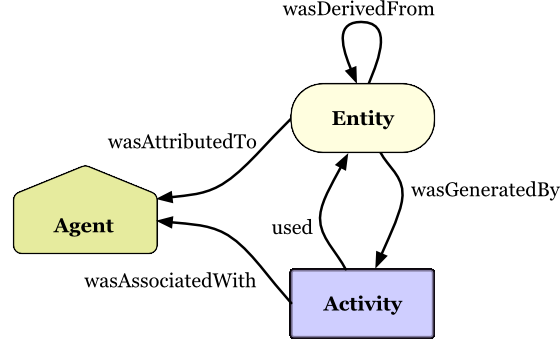
\includegraphics[width=0.5\linewidth]{images/provenance-overview}
	\caption{Example model showing the three core data types (\agent{}, \entity{}, and \activity{}) and a few of all possible \relations{} between them. 
		Taken from PROV Model Primer \cite{dsp8gil}.}
	\label{fig:provenance-overview}
\end{figure}

List of used concepts as described in PROV Model Primer \cite{dsp8gil}:

\begin{itemize}
	\item Entity, physical, digital, conceptual, or another type of `thing'.
	\item Activity, the process of instantiating or the process of changing an entity.
	\item Agent, holds (a part of) the responsibility for activities and entities.
	\item Relation, describes the interaction between two instances of the data types.
\end{itemize}

\begin{figure}[!b]
	\centering
	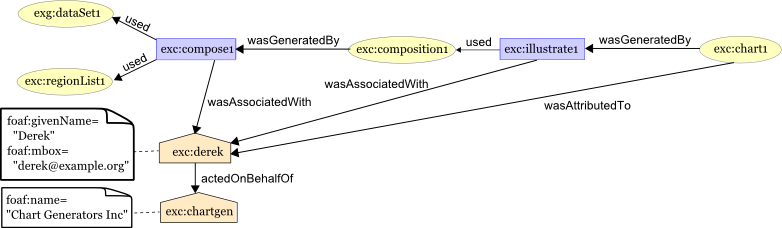
\includegraphics[width=1.0\linewidth]{images/provenance-large-schema}
	\caption{
		Real life example model which implements the model as shown in figure \ref{fig:provenance-overview}.
		This example describes the creation of a chart, the original data used, the intermediate data generated during the process, the used software, who was responsible for the work, and who this person was working for.
		An addition to figure \ref{fig:provenance-overview} is the use of \attributes{}, these are displayed with document icons and provide metadata on the object they are bound to.
		In this case that is the name and email address for one the agents and the company name for the other agent.
		Taken from PROV Model Primer \cite{dsp8gil}.
		}
	\label{fig:provenance-large-schema}
\end{figure}

%An applied provenance example is given in figure \ref{fig:provenance-large-schema}.
%This figure shows what the provenance of a certain `chart' is.
%The chart (\entity) is shown at the far right side of the figure; it was generated by (\relation) some illustration software (\activity); which in its turn used data from a composition dataset; the data was generated by composing software; two datasets were used in the process, data set 1 and region list.
%The agent executing this process is Derek (\agent), he was associated with the composing and illustration software and is attributed to the creation of the resulting chart.
%However, Derek is acting on behalf of the company chart gen (\eg{} he is a contractor or employee).
%Both agents in this example have \attributes{} assigned to them to further describe them (\eg{} the full name of the company).

Three types of assertions can be described which account to provenance: relationship (object B was retrieved by applying function X to object A), interaction (received object A, sent object B), and service state (it took three seconds to send object B after receiving object A) \cite{dsp4moreau}.
Different applications of provenance can be accomplished with these assertions \eg{} data quality, audit trail, replication recipes, attribution, and informational \cite{dsp1simmhan}.
Data quality uses the provenance metadata as a check, like described with the art example at the beginning of this subsection, the user tries to discover who did what with the data.
The same applies for an audit trail, but it is used for other ends, being able to maintain responsibilities.
Replication recipes are an extension of data quality, a user can execute the exact same steps on the same or a different piece of data to check the work or to improve on the work done.
In the case of data ownership attribution can be used to trace who should be contacted for consent on data usage.
Lastly, informational provenance helps with data discovery and providing context for data, which helps with (for example) reuse.

%Furthermore, there were three points of interest found regarding the implementation of provenance: data object identifiers, manual versus automated data entry, effect on performance.
%Data object identifiers (DOI) can be used to identify and cite data \cite{dsp1simmhan}.
%When these DOIs are used in publications the provenance can be easily gathered later when an interested party wants to check the process of an experiment.
%If provenance metadata is entered manually be users there is a high risk of losing value from missing values and non-standardised input \cite{dsp1simmhan}.
%Manual versus automated is an issue because of performance, provenance creates a overhead both in computational resources as data storage.
%Therefore, metadata should be gathered and stored on a `piecemeal basis' \cite{dsp4moreau}.

%TODO: add discussion part? How does provenance help with security?
	
	\chapter{System Design \& Implementation}
	\label{system-functionality}
	
	\section{Function Design}

During the brainstorm many functions were discovered.
As described in section \ref{brainstorm} each of them was assigned to a certain function group, \ie{} user, request, data, or publication.
With this knowledge the functions can be visualised based on simple ordering based on the groups and prospective users as seen in appendix \ref{identified-functions}.
Each of the groups describe the management needs for the specific step in the research workflow.
When also considering the workflow this simple ordering can be fitted on top of the workflow.
The result of fitting is shown in figure \ref{fig:functions-workflow} and will be described in the following paragraph.

\paragraph{Visualised}
In figure \ref{fig:functions-workflow} each of the functions belong to a certain actor (user or system), this is depicted by the colour of the actor block (light shade) and the corresponding colour of the function block (dark shade).
The function groups are exempted from this rule as they only exist to give structure to the figure.
During the brainstorm session weight was given to the requirements, functions with less need for immediate implementation are displayed greyed-out (\ie{} change data, data curation, analyse, store outcomes).

When traversing the research workflow one should start from the {\tt user} block.
From here the {\tt register} function is the first step, the researcher registers as a user of the system.
After registering the account is send to the administrator user for {\tt approval}, hence the red colour for the function block.
Etcetera.
Each of the functions are mapped out according to the following story:

\begin{quotation}
	\noindent A researcher wants to investigate a certain hypothesis on the \project{} dataset.
	He or she needs to register an account with the system which is then checked and approved by the data manager.
	
	Next, the researcher formulates a data request on the system.
	From the data dictionary the researcher searches (filter) for the appropriate data items, names of data items are called headers.
	The researcher creates the request with the necessary information that the committee needs to base their decision on.
	The system provides feedback based on user entered or detected keywords.
	Based on this feedback the researcher can edit the request or send it on for approval.
	The committee checks and approves the request.
	
	After approval the system creates a subset of \project{} data containing the requested data items.
	The researcher filters this subset and downloads a selection of the data.
	Another possible path is that the researcher prepares the data for analysis on the system and the outcomes are stored.
	
	To complete the request the researcher uploads his or her paper which is then again approved by the committee.
\end{quotation}

\begin{figure}[!htb]
	\centering
	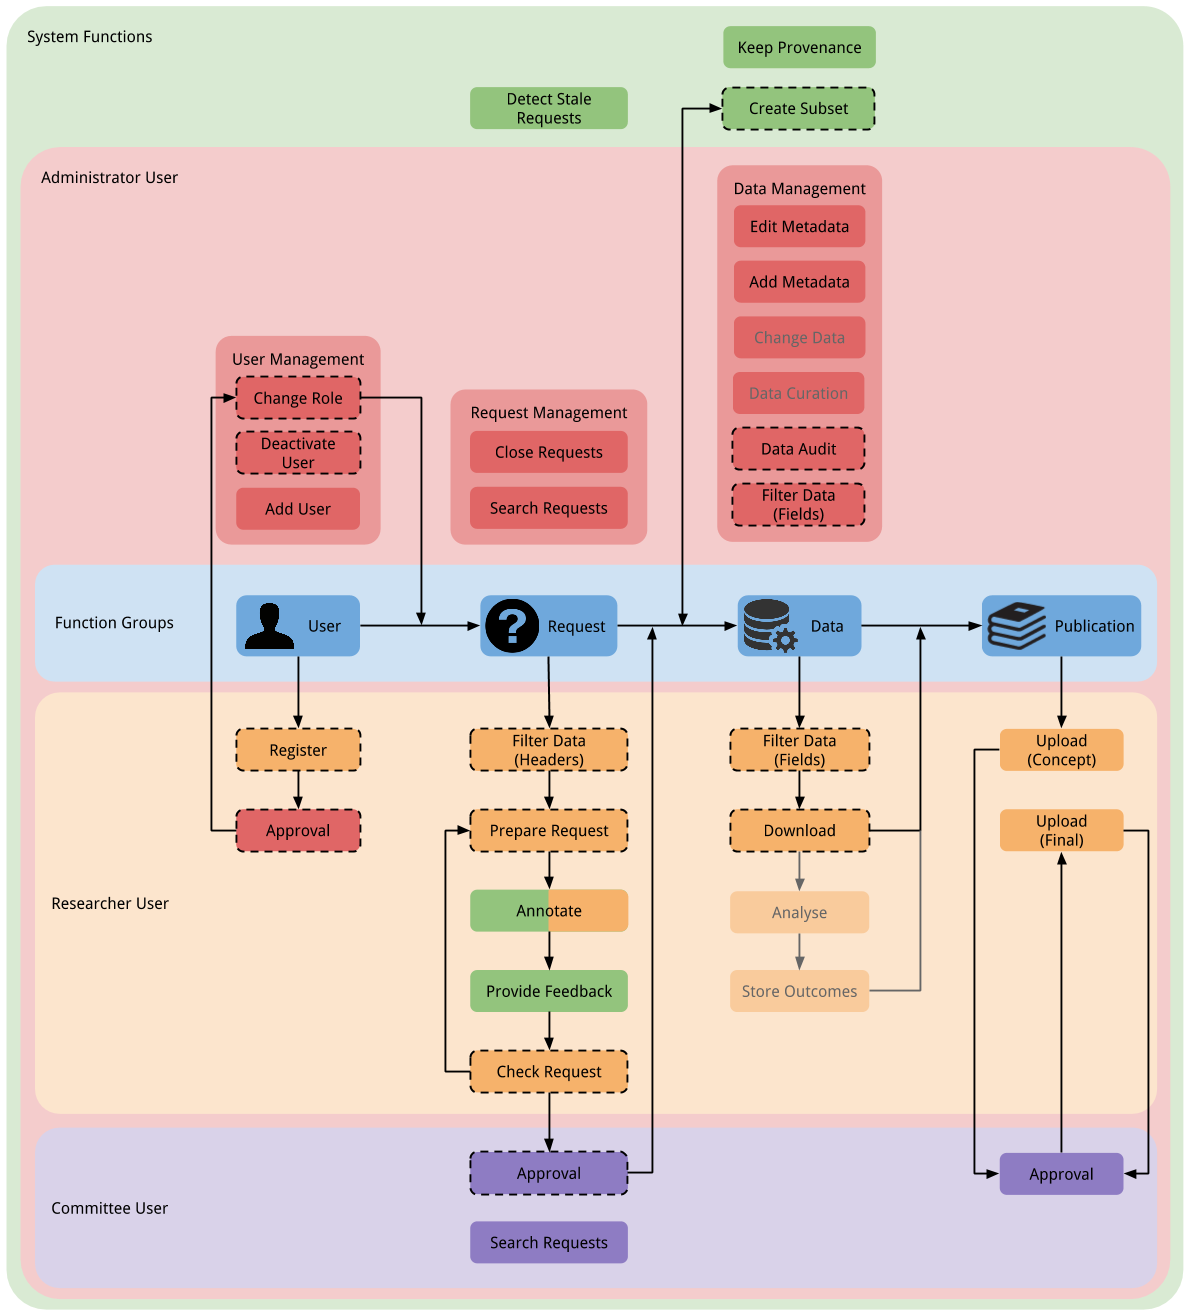
\includegraphics[width=1.0\linewidth]{images/functions-in-workflow}
	\caption{
		Mapping of functions according to function groups, actors, and research workflow.
		Vertical columns are used for function groups, colours are used for function to actor grouping, arrows are used to depict the workflow.
		Greyed-out functions are deemed less important, which was an outcome of the brainstorm session (see section \ref{brainstorm}).
	}
	\label{fig:functions-workflow}
\end{figure}
	
	\section{Re-use}
\label{reuse}

\subsection{Review}
\label{reuse-review}

For the reuse portion of this system the main criteria was data management.
This is the most significant part of the \ivfsystem{} and therefore should be well implemented.
Also implementation had to be done in a short time due to study planning restrictions.

Multiple systems were considered and evaluated.
Because extensions were needed the system preferably had to be open-source.
Three systems were included in an more in-depth evaluation, two externally developed open-source systems and one in-house project.
The external software was identified through the paper of Leroux \cite{leroux2011}.

\paragraph{External system evaluations}
The external systems identified were OpenClinica and DADOS Prospective.
Both are open-source and for OpenClinica an online demo is available.
These software packages are called clinical trial management systems, which quickly becomes apparent when using the system.
Focus lies on data entry and retrieval for low-level (researcher) users, and on research overview for high-level (management) users.
Overview meaning displaying statistics on participants and the clinics they belong to, how many inclusions were made, follow-up percentages, etc.

Per study data collection protocols can be defined, when starting a new study the definition functionality is very flexible.
After the protocol has been defined it is fixed for each of the study participants.
This is very useful in longer running (prospective) studies where collection should be standardised for quality, analysis, and reuse purposes.
In principle, as far as notable for OpenClinica, there are no features directly supporting data sharing or reuse.

\paragraph{In-house development}
A system named Rosemary has been developed in-house at the same department this study was performed at.
Handling data, applications, submissions, and input and output of these submissions is what it was build for.
The context domain is neuroscience, the data used comes from MRI machines and are mainly references to images and their metadata.
These are then submitted for processing by applications resulting in outcomes (also stored in the system) used in further analysis.

Considering the data management part, there are data input, filtering, and reuse possibilities.
Input is restricted to automated functions and there are no manual input interfaces available.
However, once data is in the system it allows for each data item to be used in access restricted subsets.

\paragraph{The better pick}
It quickly becomes apparent that no existing system is able to cover all the needed functionality, even when looking at only data management.
The decision was made to use the in-house Rosemary project for further development.
The choice is made based on several considerations.
Flexibility in the code is an important item \ie{} open-source, extensible, easy to develop.
Next to this short lines on expertise are useful for a quick development process, once a (coding) problem is encountered it can be solved in a matter of hours.
Lastly, during the evaluation process it became clear that the data model could be reused with minimal effort.
	\section{Rosemary-based Design}
\label{reuse-rosemary}


Compared to the functional design (section \ref{function-design}) the most critical part of the system, data management, is mostly covered by Rosemary.
Datasets are bound to \emph{workspaces}, which have an owner and members that can all view the data inside, effectively restricting data access.
To enable  search and filtering, a specific model for raw data storage is used and supplemented with an extensive tagging system.
The flexibility of this system means that part of the request and the whole data management requirements can be implemented with minimal changes.

User management can be totally reused, but it will need extensions to provide for the necessary user roles.
Furthermore, request and publication management will need to be introduced into the system.

\begin{figure}[!hb]
	\centering
	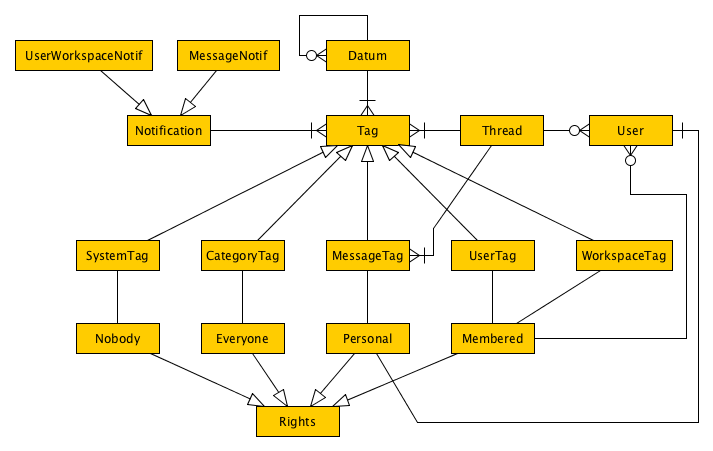
\includegraphics[width=1.0\linewidth]{images/datamodel-clean}
	\caption{
		Rosemary data model with domain specific items removed.
		Describes the workspace, tagging, datum, and notification models.
		The unedited Rosemary data model can be found in appendix \ref{unedited-datamodel}.
	}
	\label{fig:reuse-rosemary-dm}
\end{figure}

\silvia{i believe that from here you actually describe the prototype. keep clear what was rosemary, what is new, or what has been adapted. maybe it is not so relvant to stress the differences, but to have a complete and understandable explantion of what you have done}
\paragraph{Data model}
Figure \ref{fig:reuse-rosemary-dm} depicts the Rosemary data model where the (\ie{} domain specific) items are removed.
%A full view of the data model can be seen in appendix \ref{unedited-datamodel}.
Implementation is done in mongoDB, a document-oriented database \cite{}.
\silvia{present the main entities of the model here. the figure should stay in the body}
The data model and its implementation provide some interesting possibilities.
%What is described in figure \ref{fig:reuse-rosemary-dm} 
A {\tt Datum} is a single piece of raw data, \ie{} a row in a relational database.
This data can be tracked and reused endlessly by applying a {\tt Tag} object.
For example, access control can be applied by tagging a {\tt Datum} with a {\tt WorkspaceTag} which is owned by a {\tt User}.
Many different constructs of this sort can be achieved without ever touching the structure of the actual model itself.
The reuse in the \ivfsystem{} relies heavily on this concept, which means only slight changed had to be made to the original data objects.
	
	\section{Implementation}

\subsection{Processes}
\paragraph{Division of management tasks}
Describe user, data, request, and publication-management, which were implemented and which were left out for now.
What functions for each of the tasks was implemented.

\paragraph{User roles}
What user roles were implemented and which (parts) of the management tasks are they allowed to perform.

\paragraph{Security}
Talk about security story and provenance.
	\subsection{Rosemary}
\paragraph{Testing the data model's flexibility}
How was the Rosemary data model changed to fit to our functional needs.
Show figure with differences.
\paragraph{Back-end and front-end}
Explain how the front and back-end were changed to meet each of the functions.
	
	\chapter{System Evaluation}
	\label{evaluation}
	
	\section{Case Evaluation}

\subsection{Set-up}
\label{evaluation-setup}

\begin{figure}[!b]
	\centering
	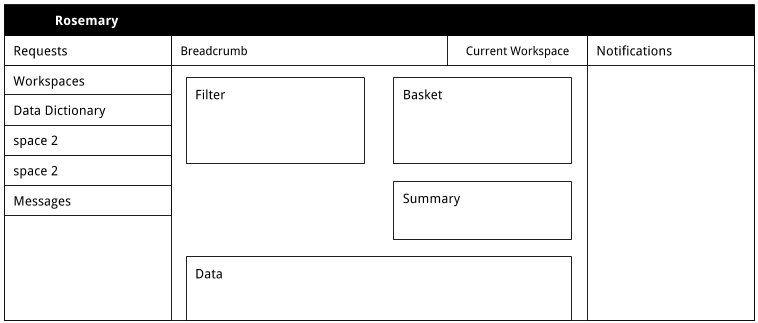
\includegraphics[width=1.0\linewidth]{images/evaluation-layout}
	\caption{
		Wireframe of the Rosemary layout, showing the data management features: filter, view, select.
	}
	\label{fig:evaluation-layout}
\end{figure}

All evaluations were done in an informal open-talk setting with no predefined questions.
First, the purpose of the meeting was explained in a few sentences.
Each user had to perform tasks according to the assigned case: researcher, committee, administrator.
There were three testers, some were assigned two cases as they both fit in the field of experience of the user.

Tasks were described according to the system schema from the brainstorm section (see section \ref{brainstorm}, figure \ref{fig:brainstorm-after}).
The interviewer only gave directions after the tester indicated that they did not know how to proceed.
If the tester struggled with a task the interviewer tried to encourage the tester to think aloud.
From this the process bottlenecks and design flaws of the system were identified.
Also, testers were asked to provide design or process alternatives.

The following cases are loose transcripts of the evaluation sessions.
Identified problems and possible improvements are summarised in the analysis section.

\begin{figure}[th]
	\centering
	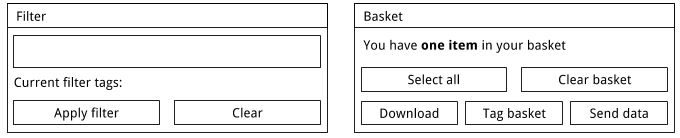
\includegraphics[width=1.0\linewidth]{images/evaluation-basket-layout}
	\caption{
		Wireframes of the Rosemary filter and basket layout, showing the search and select data management tools.
		These wireframes are the more detailed versions of the filter and basket blocks shown in figure \ref{fig:evaluation-layout}.
	}
	\label{fig:evaluation-basket-layout}
\end{figure}

\subsection{Cases}
\label{evaluation-cases}

In the following cases refer to figure \ref{fig:evaluation-layout} for clarification on the used terms.

\paragraph{Researcher}
From all the cases this is arguably the largest as it has the most extensive (implemented) functions.
Therefore, all the testers performed the researcher tasks to find more flaws or give more support to flaws found with both testers.
The tasks that had to be performed were: search the data dictionary for headers, use these data headers in a request, download the request data.

%Finding the data dictionary was not a big problem for the testers, however it was unclear that the dictionary itself was (like all data views) a workspace.
%Having a separate workspace for each of the requests made sense but the dictionary should be a entity that exists on itself.

Finding the data dictionary was not a big problem for the testers.
The next step is filtering, this is relatively easy as the input (see left side of figure \ref{fig:evaluation-basket-layout}) is text based and the search itself is fuzzy.
Dictionary items can be sought for based on name, description, and keywords.
Because in the prototype the descriptions are nonsense it was difficult to find the wanted data headers.
Two of the testers did not notice that the search is instantaneous (like google search).
This resulted in pressing enter and clicking the `apply filter' button multiple times before noticing that the data had already changed at the bottom of the screen.
One of the testers prefers to search the data analogically (\ie{} print the data) and later select the wanted items in the interface.

The filter function plus the nonsense data made it rather hard for the testers to find the desired headers, they were asked to select a couple of random headers to start a request with.
Selection was straight-forward but the testers did not notice that selected items were added to the `basket' (see right side of figure \ref{fig:evaluation-basket-layout}).
Therefore, two asked `how do I keep this selection when I start searching again?'.
This also resulted in two of the testers using the `select all' function on the basket. 
Clicking this will make a selection of \emph{all} the items in the workspace, basically overwriting the previous basket and losing all the progress.

To proceed in the task of making a request the testers looked for a button on the basket.
However, the buttons (see right side of figure \ref{fig:evaluation-basket-layout}) are specific to a raw data view and do not make sense in a dictionary view of the system.
The testers needed to be explained that the basket is kept in the back of the system and can be used over multiple views.
Clicking the request button at the top left of the screen is the correct action, then selecting `new request' results in a form with the basket attached to the end showing which items were selected.

Data download is straight-forward, this is done by going to the correct workspace from the menu on the left, selecting the wanted items (or select all), and clicking the `download' button.
No problems were found here, however one of the testers noted that in principle \emph{all} data will be downloaded every time.

\paragraph{Committee}
The committee tasks are the shortest as the list contains one function: request approval.
Viewing requests that are ready for approval is done by selecting the `request' button from the left menu.
Now a list is shown of all these requests and the data that is necessary for making the decision.
Approval is given (or not) by selecting a approve or disprove button, a vote remains open for change until all committee members have casted their vote.
What vote was cast is shown both with a symbol (V/X) as with a colour (green/red) which was directly clear to the tester.

Communication functions are build into the view, clicking a request redirects to a `new message' view which already has all affected committee members in the `to' field.
There was a suggestion to add a comments thread to the request itself instead of the separate message construction.
Furthermore, the redirect was confusing for the tester as the expectation was that it would lead to more information on the request.

\paragraph{Data administrator}
Lastly, the data administrator performed the user management functions.
The user overview is not complex in functionality, a list of users is shown.
Each with buttons to perform the following actions: make committee member, make active, approve.
This was clear and would be easy to use in a real-life scenario.
However, the tester noted that there are some process flaws.
If one of the users of the system changes institutions most of the time the data manager is not informed, this is left to the P.I.s.
Therefore the system should contain support functions for non-administrators to view the list of users and communicating with the data manager about what actions should be taken.
	%\paragraph{Summary}
\section{Summary}
\label{evaluation-summary}

As with brainstorming creating a user interface is not an exact science.
For evaluation ends design heuristics are used, and the found problems can be mapped against these.
The used list is from Nielsen \cite{designHeuristics} and contains ten famous heuristics:

\begin{enumerate}
	\item Visibility of system status;
	\item Match between system and the real world;
	\item User control and freedom;
	\item Consistency and standards;
	\item Error prevention;
	\item Recognition rather than recall;
	\item Flexibility and efficiency of use;
	\item Aesthetic and minimalist design;
	\item Help users recognise, diagnose and recover from errors;
	\item Help and documentation.
\end{enumerate}

\noindent{} Based on the system's process and the potential as a supporting factor in doing research the system got positive feedback.
One of the testers mentioned that the system as a prototype might be used for demoing purposes.
Relatively simple functions from the system can show that thought went into the workflow of data security.
Thereby fulfilling the goal of persuading data deliverers and providing more trust.

The biggest hit is the request management process.
From multiple perspectives the system can show what requests are in progress and information is available to make request `dashboards' for management purposes.
Which also brings possibilities for monitoring by data owners.

Design-wise the data view is a perfect example for the user freedom and flexibility heuristics.
There are three ways of viewing namely: raw data, graph, aggregated.
The user may switch between these views and can pick whichever they prefer for their current task.
On the other hand, the fact that the data view does not support (analogue) printing of data shows lack in flexibility.

There are things to clean up, most of the encountered problems can be related to the system status visibility.
For example, when the user is in the data dictionary the buttons on the basket do not account for this.
Which means that two out of the three buttons are completely out of context for what the user is doing.
System visibility problems are also reflected in the fact that testers tried to `start' the search by hitting enter and not noticing that the results had already updated.
Lastly, selecting data and putting it in the basket caused confusing meaning that the purpose of the basket is not well understood.

As for the heuristic `recognition rather than recall' a few issues were found as well.
The `select all' function on the basket confused the user, thinking they would select all data which was already \emph{in} the basket.
Clicking this button made the user loose all progress made resulting in a problem with recognising and recovering from errors.
Also, going from a basket selection to preparing a request was unclear as they were looking in the wrong place.
Lastly, the redirect from request overview to new message was unexpected behaviour.
	
	\chapter{Discussion \& Conclusion}
	\label{discussion}
	
	Below we present ...
\silvia{explain the rationale to organize the topics as you have. also important to distinguish discussion (you are free to discuss whatever you want) and conclusions (you can only conclude things for which you have evidence)}

\section{Summary}

In the Netherlands about 5\% to 8\% of all couples remain childless due to infertility or subfertility.
There are several treatments used to assist in reproduction, for example IUI, IVF, and ICSI.
While it is known how many treatments result in a pregnancy, it is relatively unknown what the outcomes are for children born out of these pregnancies.
For this end the \project{} was started: to gather and analyse data from both the fertility clinics as the national birth registry (\ie{} \PRN{}).

Because considerable effort went into data gathering, data management should be supported to get the most gain out of this valuable data set.
From this vision, the idea for the \ivfsystem{} was formulated.
Initially no data was available, which made requirement analysis with stakeholders a difficult process.
A study was performed, resulting in an initial system concept that was then used as input for the brainstorm session with stakeholders.
During the session it appeared that there are many more aspects which should be incorporated into the system, 
the most important aspects of which concerning data reuse.
Identified requirements were separated into different management groups: user, request, data, and publication.

Data management is the most extensive requirement group, thus four existing information management systems were evaluated for potential reuse.
An in-house developed project, Rosemary, was chosen as a development starting point for the \ivfsystem{}.
With minimal changes to the data model, it was possible to store and use the \projectdata{} within the Rosemary framework.
Due to time restrictions the functions for user, request, and data management were partially implemented.
Publication management functions were not addressed by the implemented prototype.

During the evaluation of the prototype with users, it became clear that for a successful demo more polishing of the system's workflow (\ie{} the manner in which a user moves through the system) is needed.
Also we estimate that one or two iterations of user-centred design should still be applied to remove most of the fundamental confusions in the interface.
\silvia{security?}

\section{Discussion}

\paragraph{Gathering the \projectdata{}}
%What are the biggest blocking factors in doing research with sensitive data and how can these be overcome?
%What needs to be changed in the current attitude towards data usage to promote big data in a IVF medical domain?

In this study the \projectdata{} is considered `fixed' and would be delivered by the \project{} at the start.
Data gathering should be outside the scope of this study.
However, data was not available, causing problems with development as described in chapter \ref{requirements}.
It was decided that the gathering would be a joint effort with other participants of \project{}.
The experiences and impressions during the data gathering process are described below.

Data gathering hurdles are encountered roughly in the following order.
Firstly stakeholders at the fertility clinics have to be persuaded to cooperate in the study.
This is done by explaining the goal of the study, the study protocol, and data contract (\ie{} for what purpose is the data gathered and how will it be used).
Then the protocol and contract have to be evaluated by an ethical committee.
Each clinic has its own ethical committee, thus the documents are evaluated for each clinic individually.
When permission is granted to deliver the data there is the question of who is going to gather the data.
Some clinics have data managers, but others required the \project{} researchers to gather the data themselves.

The last (technical) step in the process seemed more complex than anticipated, and significant support was needed by the \project{} researchers to obtain the data.
%When data managers collected the data the delivered datasets are neatly structured and clean.
%Researchers from the \project{} were not equipped with the necessary expertise to collect datasets from the clinics that did not deliver themselves.
%We helped the data gathering by giving technical advice and creating data queries.
There are thirteen fertility clinics in the Netherlands with a wide range of electronic patient records (EHRs).
Luckily during the \project{} most clinics were switching to a standardised EHR from a single vendor.
%Therefore, one data query could potentially be used at multiple clinics.

The first problem encountered was intellectual property restrictions.
Researchers could not get access to the data dictionary of the EHR.
Therefore, trial and error with existing queries, four visits with an expert fertility clinician, and approximately 50 query versions were needed.
Also, due to the accessible data dictionary the query could not be fully optimised which resulted in `dirty' data.

Furthermore, the EHR could be implemented on database software from two different vendors (Microsoft or Oracle).
Queries (executed from within the EHR) written for one of the vendors did not work for the other.
Therefore, the query had to be translated and debugged again.

\silvia{i have the feeling that from here you go back in time, to the phases that came BEFORE the technical phase. Also, was it one year or six months. the text below is confusing}

The actual gathering took about six months.
Even though at the start of the project many heads of clinics were enthusiastic, the preparation steps took much longer, about one year.
Many decisions had to be taken and certainly the ethical committee evaluation can take quite some time. 

Stakeholders will try to protect the interests of the clinic.
A strict limitation was set that no comparison between clinics would be done with the \projectdata{}.
Furthermore, during the security review (appendix \ref{security-appendix}) the following quote was found in literature: ``They [clinicians] wanted to help achieve these benefits, but also wanted to be sure that patients' rights were protected and that clinicians were not in danger of breaking patient confidentiality and the law''.
We assume that the same holds in the case of the \project{}.
This leads to the impression that the real consideration for stakeholders is related to control over their data.

Currently each data request is evaluated by the data owner, which gives them great control over who they deliver data too.
Furthermore, data has value that can be monetary but also academic (\ie{} scientific value in the form of potential publications).
Gathering data and putting it in a repository weakens (or removes) ownership of the data and the owner loses the potential profits.

To summarise, technically there are a lot of issues to overcome, \eg{} data is geographically spread, restrictions by intellectual property, or there is no standard data model.
But what took the most time in the \project{} data gathering was to go through the bureaucratic process.
This stresses the notion that data should not be discarded after the project ends, but should be reused.
Moreover, we think that a \ivfsystem{} can give back control and trust to the data owners,
potentially making them more willing to deliver data and thereby shortening the bureaucratic process.

\paragraph{Supporting reuse}
%How do we implement a user-friendly system in a IVF medical domain which covers problems concerning: data security, data access, data browsing, and data querying?

During the development process some interesting changes occurred.
The focus of the \ivfsystem{} changed during the requirement discovery phase (see chapter \ref{requirements}) as explained below.

Originally the idea was to support researchers in doing their research.
The initial system concept (section \ref{process-analysis}, figure \ref{fig:brainstorm-before}) describes functions aimed at researchers such as data querying and data analysis.
We assumed that these functions would be important for our prospective users.
During the brainstorm session (section \ref{brainstorm}) many hurdles in the current research workflow came to light.
Normally these might be hidden to spectators as workarounds are used.
The most critical for the \ivfsystem{} is the need to support data requests for datasets like the \projectdata{}.
Moreover, the stakeholders representing the researchers said that data analysis was an rather uninteresting feature (\ie{} a `could have').
This in contrary to the vision put forward by big data literature about the benefits of computerised decision making and data mining (see chapter \ref{introduction}).

With the focus on data requests, also a new user of the system was introduced, namely the committee member (section \ref{brainstorm}, figure \ref{fig:brainstorm-after}).
These users are key stakeholders from each clinic which supplied data to the \projectdata{}.
Requests are presented in a transparent way and evaluated.
Data is only delivered when the committee members give permission,
thereby partly giving the ownership back to the data owner.
This links back to the impression from that bureaucracy of data gathering is a lengthy progress partly because of ownership and interests.

Implications for the \ivfsystem{} are that, instead of supporting researchers in doing their research, the system is now more of a data reuse management system.
Reuse of sensitive data is a difficult problem as there are many aspects to take into account.
One of the most important aspects for sensitive data is security (see section \ref{security-summarisation-analysis} and appendix \ref{security-appendix}).
It is known that when humans are involved errors are inevitable when time goes by.
Providing overviews and insights in the process they are working with can achieve error prevention and facilitate trust building.

As shown in the development of the \ivfsystem{} multiple actors are involved in the data management process.
A lot of communication will occur between these actors, which currently (without the \ivfsystem{}) are mostly done asynchronously and partly off-line.
Providing the actors with a communication channel keeps the conversation encapsulated in a single system.
This dataset can be leveraged to provide managers with insight in the process and can help them spot possible errors and prevent these.

When making data reusable it is hard to check whether  the right references are used in publications.
On the other hand, data reuse can lead to better research, for example publications can be checked by an independent institute.
With a \ivfsystem{} data can be restricted, whereas the line of communication between data owner and consumer remains short.
This will bring all the benefits of data reuse while the data owner still has a grip on what happens with it.

Lastly, as one of the system's testers noted (section \ref{evaluation}): the system can be used as a demo.
Next to data providers, institutions providing grants are highly important and interested in data reuse.
Nowadays they require that their investment in data gathering should lead to high returns for the scientific community.
This statement is also supported by big data literature, as presented in chapter \ref{introduction}.
Mostly this means that data reuse is of high priority, and the \ivfsystem{} can show exactly how the \project{} consortium could provide this.

Summarising, the system's goal audience changed from researchers to committee members (or data owners).
While the purpose changed from doing research to managing data reuse.
Lastly, the prospective users of the system see it as a opportunity for showcasing their intentions considering data reuse towards funding institutions.
This is interesting because there are currently no other systems which provide these functions.

\paragraph{Extrapolate to other domains}
%How can this specific system be used in other settings/knowledge domains?

The previous section argued the benefits of the \ivfsystem{}; however, it is specific to the domain of the \projectdata{}, \ie{} \IVF{} and \PRN{} data.
Now we will discuss how the system might be used in other domains.

It is a good idea to work towards a modular solution that implements core elements of user, data, request, and publication management.
Different domains can pick what they need from these modules and add their specific `sugar'.
For simplicity we will split the whole process into two parts: data gathering and data reuse.

There are other projects that aim at building towards something similar as the \ivfsystem{} (\eg{} the Yoda project \cite{yodaGithub, yodaPresentation}).
The scope of these projects is much broader, as they include data gathering and data reuse (among possible other aspects).
Also, no complete system exists today yet.

Multiple systems exist which perform data gathering (and management) functions, 
for example, OpenClinica and DADOS prospective.
Of course there are many more systems that perform about the same functions (see section \ref{evaluation}).
For the sake of this section all these systems will be considered as Clinical Trial Management (CTM) software.

Each of the reviewed CTM systems in section \ref{evaluation} at least provides data gathering and data retrieval functionality.
Most of them implements gathering with flexible input form creation which, after defined, are to be strictly followed during a certain trial.
Data retrieval (mostly) consists of a downloadable formatted file of the data, specific for statistical packages like SPSS.

In CTM software data may be shifted around by adding other users as members of a dataset.
However, data reuse as defined in this study cannot be fulfilled with this functionality.
The \ivfsystem{} can deliver these functions.
When handling data gathering and reuse as two separate parts, it becomes easier to implement in different domains.
CTM software might be used for data gathering, and when the dataset is complete it is exported to the \ivfsystem{} to enable reuse.
We believe that the abstraction of the data model implemented in the \ivfprototype{} is so generic that almost any type of data could be fit with minimal changes (see section \ref{implementation}).
	
	\section{Appraisal}
\paragraph{Strengths and limitations}
One registry as example (no branching to other domains). 
Limited time to program, thus less implemented functionality.
However, this example provides many different angles to approach the problem.
\paragraph{Comparison with existing systems}
Comparison with other existing software (OpenClinica, etc)
\paragraph{Future research and development considerations}
What functions need to be implemented to give the system an extra `boost'.
How can the system manage the expectations of users better.
How can the system better support users in their data management tasks.
	
	\section{Conclusion}
\allard{TODO once position paper is done}

%\begin{enumerate}
%	\item How do we implement a user-friendly system in a IVF medical domain which covers problems concerning: data security, data access, data browsing, and data querying?
%	\item What needs to be changed in the current attitude towards data usage to promote big data in a IVF medical domain?
%\end{enumerate}
%
%\begin{itemize}
%	\item What are the functions of this system and which parts of the research process should this system support?
%	\item Who are the users and what are the use-cases for these users?
%	\item What are the legal and security aspects of this system?
%	\item What is the data model for this system?
%	\item What functions were actually implemented in the prototype? \silvia{this is no research question. maybe 'what is a minimum prototype to demonstrate ...'}
%	\item To what extent does this system meet the expectations of users?
%\end{itemize}
%
%\begin{itemize}
%	\item What are the blocking aspects of data usage?
%	\item What are the promoting aspects of data usage?
%	\item What alignment needs to take place to promote data usage?
%	\item How can IT be leveraged to achieve this goal?
%\end{itemize}
	
	\chapter{Data Management Position}
	\label{position}
	
	\section{Introduction}
\paragraph{Problem}
Describe data `usage' phases and what the problems are now:
\begin{itemize}
	\item Study preparation, data usage approval
	\item Data retrieval
	\item Data massaging/preparation
	\item Data analysis
	\item Data reuse
\end{itemize}
\paragraph{Position}
There should be more data re-use and cooperation between data producers/consumers.
IT can help with the alignment of these two factions.
	
	\section{Background and Evidence}
How is research performed now?
Describe Dutch law on privacy and data usage.
Explain how METC and commissions influence data usage.
Talk about clinicians.
Patient willingness to share their data for research.
Big data and its general stance on data usage.
	
	\section{Discussion}
(Limitations):
\begin{itemize}
	\item How does Dutch law prescribe security and ethics to be taken into consideration and why does this matter, what is the fear?
	\item Is law taken into account in the right manner every time?
	\item How do METC, commissions, and other influential bodies limit the use of data?
	\item What are the clinician's opinion, thoughts, and `holding back' in fear of rebuttal
	\silvia{what is rebuttal here?}
	\item What are expected hold-ups for research now (data gathering can take extremely long)?
	\item Will patients withhold their data for use in research and why?
\end{itemize}
(Chances):
\begin{itemize}
	\item What does existing big data research describe is necessary in order to conduct successful and meaningful studies?
	\item What are some necessities for a certain fluidity in using sensitive data for research?
	\item \silvia{How to can?} limitations be aligned with the big data opportunities
	\item What needs to be changed in attitude in order to open up data reuse and sharing (introduce Scandinavian ideas)?
	\item How can online and offline (IT) be leveraged to bring convincing and easy-to-grasp ideas to inspire people to change their way of working?
\end{itemize}
Give both sides of the issue and discuss how these two can be aligned with each other to meet at a sweet spot for both factions.
	
	\section{Conclusion}
\paragraph{Further steps}
Figure out if IT can be leveraged to align medical and technical personnel.
\paragraph{Proposing solutions}
IT leverage in the form of a system (like the one in this thesis).
	
	\clearpage
	
%	\printbibliography
	
	\appendix
	\chapter{Abbreviations}
	\label{abbreviations}
	
	\paragraph{\IVF{}} \\
In Vitro Fertilisation, an assisted reproduction technique.
In this paper also used to denote the medical domain of fertilisation.

\paragraph{\PRN{}}

\paragraph{\project{}}

\paragraph{\projectdata{}}

\paragraph{\ivfsystem{}}

\paragraph{\ivfprototype{}}

\paragraph{CTM}
	
	\chapter{Brainstorm Schemas}
	\label{brainstorm-before-after}
	
	\begin{sidewaysfigure}
    \centering
	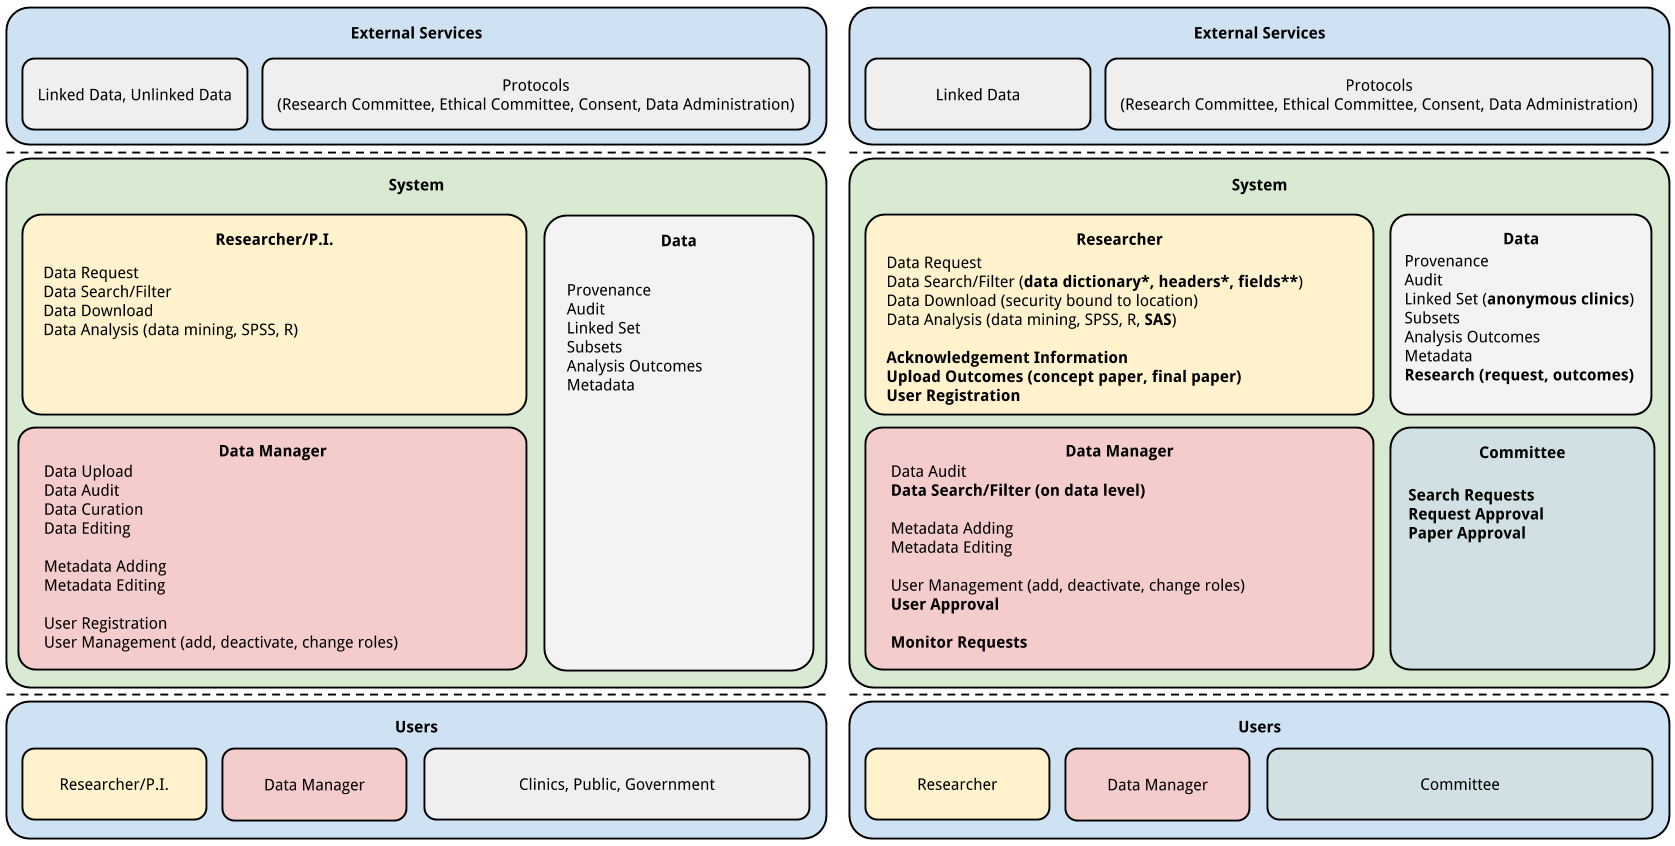
\includegraphics[width=1.0\linewidth]{images/brainstorm-before-and-after}
    \caption{
    	Side by side comparison of system functionalities before and after brainstorm as described in \ref{requirements}.
   	}
    \label{fig:brainstorm-before-and-after}
\end{sidewaysfigure}
	
	\chapter{Security Checklists}
	\label{security-appendix}
	
	\section{Checklist A}
\label{security-checklists-a}

This section gives two checklists found in the literature.
These lists give a number of points which a system should comply to in order to be secure in the sense of privacy.
The first list describes items used to test safety of the implementation of a patient-centred eHealth solution in Dehling \cite{s17Dehling2014}:
\begin{itemize}
	\item No unauthorized person must be able to access patients' information;
	\item The real identity of patients must not be revealed;
	\item Access must be limited to necessary information and data segregation must be ensured;
	\item Unnecessary access rights must be revoked;
	\item It cannot be possible to force patients to reveal information they do not want to reveal;
	\item Eavesdropping has to be prevented during transmission and storage;
	\item It must not be possible to reveal relationships between items through observation;
	\item It must be ensured that information content is as intended and not unintentionally changed;
	\item Up-to-date information must be available whenever needed;
	\item Redundancy must be employed to ensure that data can be restored;
	\item It must be possible to store information as long as it is required (even a lifetime or longer);
	\item It must be possible to restore lost information to a specific point in time;
	\item Failure of single nodes must not impede the performance of the whole service;
	\item Systems have to be adaptable to changing performance needs;
	\item There cannot be a significant delay between data entry and dissemination to patients;
	\item Accesses to and uses of information must be attributed to the respective party and it must not be possible to deny such actions afterwards;
	\item Relevant activity (e.g. document accesses) must be logged;
	\item It must be determined who is using the software and verified that they are who they claim to be;
	\item The boundaries of trusted access to the information system must be known and controlled;
	\item Unintended actions and/or activity must be detected;
	\item Unauthorized access must be avoided and access rights must be managed;
	\item Impairment of hardware (theft, natural disasters, ...) has to be prevented;
	\item System vulnerabilities must be detected;
	\item Important information has to be easily accessible;
	\item Patients have to be able to control who can access what information;
	\item Authorization details must be substitutable (loss, technological obsolescence);
	\item User ethics, obligations, and proficiency must be reinforced;
	\item In case of emergency, medical professionals must be able to access required information;
	\item Patients have to agree to uses of their information and patient consent must be managed;
	\item Patients have to be able to retrieve information stored on them.
\end{itemize}

\section{Checklist B}
\label{security-checklists-b}

The second list describes questions used to test EHR systems on security and privacy in Fernández-Alemán \cite{s8FernandezAleman2013}:
\begin{itemize}
	\item What standards and regulations does the system satisfy?
	\item Does the system use pseudo anonymity techniques?
	\item Is the user data encrypted? 
	\item What authentication systems are used? 
	\item Can access policies be overridden in the case of an emergency? 
	\item If the system needs user roles, who defines them? 
	\item Who grants the access to the data? 
	\item What kind of information is exchanged? 
	\item Are there audit logs?
	\item Are the systems' users trained in security and privacy issues? 
\end{itemize}
	
	\chapter{Identified Functions}
	\label{identified-functions}
	
	\begin{figure}[hb]
	\centering
	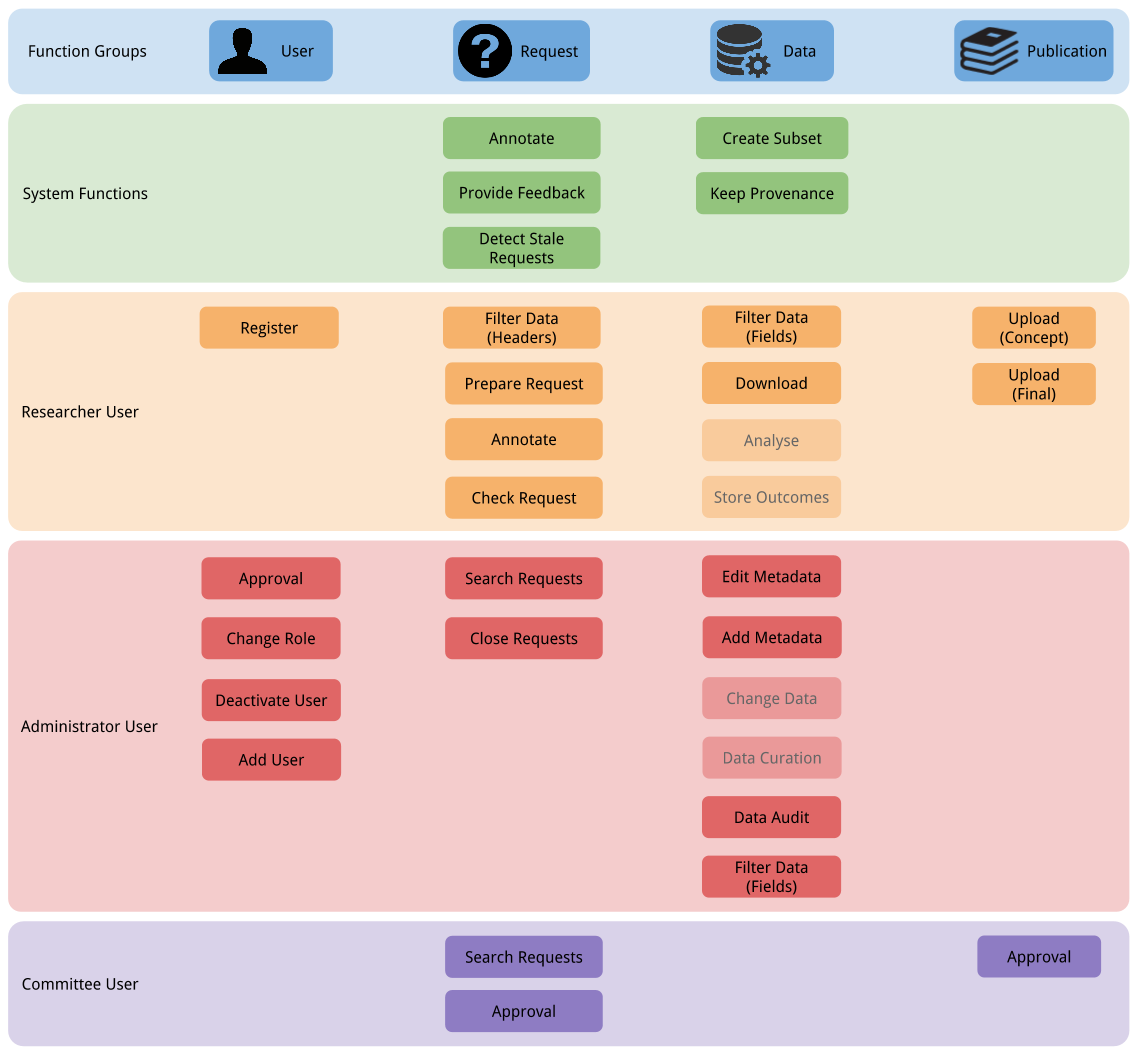
\includegraphics[width=1.0\linewidth]{images/functions-in-groups}
	\caption{
		All identified functions grouped by the four function groups.
		Underlying requirement analysis described in \ref{brainstorm}.
	}
	\label{fig:all-functions-grouped}
\end{figure}
	
	\chapter{Unedited Rosemary Data Model}
	\label{unedited-datamodel}
	
	\begin{figure}[ht]
	\centering
	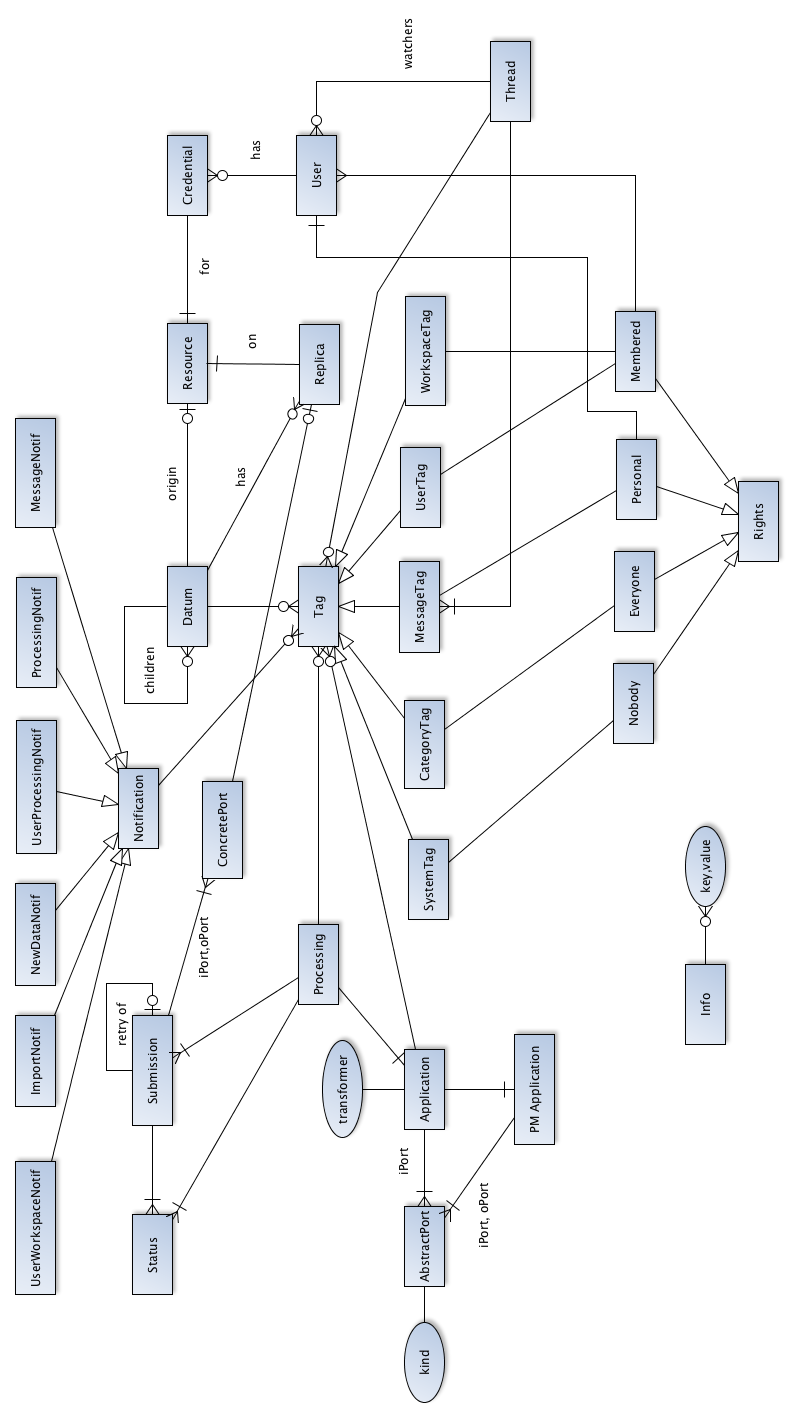
\includegraphics[width=0.54\linewidth]{images/datamodel-unedited}
	\caption{
		The full unedited data model as implemented in the Rosemary project \protect\url{https://github.com/AMCeScience/Rosemary}.
		Describes the workspace, tagging, application, submission, datums, and notification models.
		Taken from \protect\url{https://github.com/AMCeScience/Rosemary/blob/master/docs/general/rosemary-dm.png}.
	}
	\label{fig:unedited-rosemary-dm}
\end{figure}

\end{document}
